\chapter{Introduction}
Space is obviously quite important for physics. Finding a mathematical model for space presents some challenges. Many branches of mathematics have tried to model essential characteristics of space in different ways. This has lead to many different mathematical meanings, one of which we have already seen: the vector space.

\begin{displayquote}
SPACE. The word came into English—from Old French from Latin—around 1300. The OED entry distinguishes many meanings. In one sense (under heading 6b) it has room as a synonym. This word derives from the Old English and is related to the modern German Raum. Under heading 17 the OED defines “a space” as “an instance of any of various mathematical concepts, usually regarded as a set of points having some specified structure.” Among the quotations is a nice one from 1932: “The word ‘space’ has gradually acquired a mathematical significance so broad that it is virtually equivalent to the word ‘class’, as used in logic.” (M. H. Stone Linear Transformations in Hilbert Space p. 1.) The space age was well under way by 1914 when Hausdorff’s Grundzüge der Mengenlehre (Fundamentals of Set Theory) gave axioms for a METRIC SPACE (metrischer Raum) and for a TOPOLOGICAL SPACE (topologischer Raum).\footnote{From \textit{Earliest Known Uses of Some of the Words of Mathematics}, \url{http://jeff560.tripod.com/s.html}}
\end{displayquote}

The main branch of mathematics that is relevant for the modeling of space is obviously geometry. Just like the word ``space'', the label geometry is applied to many parts of mathematical reasoning.

\section{Erlangen programm}
In 1872 Felix Klein proposed his \udef{Erlangen programm} (named after the University Erlangen-Nürnberg, where Klein worked) which attempted to classify different geometries based on symmetries. In particular it allowed geometry to be viewed as the study of properties of figures that remain invariant under a certain group of transformations. So for example, in Euclidean geometry may be viewed as the study of properties that remain invariant under isometry transformations (these can roughly be viewed as the translations and rotations). Two shapes are called \udef{congruent} if there is an isometry that maps one onto the other. If we take a rectangle, its corners will always be $90\si{\degree}$ angles no matter how we rotate or translate it. Angles are in general invariant under such transformations. Other invariants include
\begin{itemize}
\item Distances;
\item Areas;
\item Volumes;
\item Whether lines are parallel, or not;
\item Whether points are or other shapes, or not;
\item Whether points are collinear, or not;
\end{itemize}

Another important aspect to the Erlangen program is its hierarchical nature: if we take a larger group of transformations, then fewer aspects will invariants of all the transformations. Conversely, if we restrict the group of transformations, more aspects will be invariants. For example, the isometry transformations are part of a larger group of transformations called affine transformations. In particular they are the affine transformations that preserve distance. Of the bulleted list of invariants above, the last three are affine invariants, but the first three are \textbf{not}.

In this way projective geometry may be seen as the underlying, unifying frame. Restricting it a bit we get affine geometry; restricting it a bit more we get Euclidean geometry.

\section{Analytic–synthetic distinction}
TODO

\chapter{Euclidean and related geometry}
\section{Axiomatic (or synthetic) Euclidean geometry}
Historically it was easy: geometry was the study of shapes, either on a flat plane or in space (or what was somewhat naively thought to be space). By the third century BC Euclid had published his \textit{Elements}. In it he gave gave the postulates of what is now called Euclidean geometry. Euclid held his postulates to be self-evidently applicable the the actual, physical space in the real world.

\subsection{Euclid's \textit{Elements}}
There are 13 books\footnote{It must be remembered that in ancient times book binding technology was not as advanced and works were published in smaller subunits called \textit{books}. Each book was only a few dozen pages long, in today's pages, but published on scrolls.} in the \textit{Elements}.
\begin{itemize}
\item Books I to IV and VI discuss planar geometry.
\begin{itemize}
\item[\textbf{Book I}] lays out the fundamentals of planar geometry involving straight lines.
\item[\textbf{Book II}] contains propositions to do with squares and rectangles. This has a strong link with geometric algebra due to the link with the squaring of a number.  
\item[\textbf{Book III}] lays out the fundamentals of planar geometry involving circles.
\item[\textbf{Book IV}] deals with the intersection of circles and rectilinear figures.
\item[\textbf{Book VI}] discusses similar figures.
\end{itemize}
\item  Books V and VII-X deal with number theory, with numbers treated geometrically as lengths of line segments or areas of regions.
\item Books XI-XIII concern solid geometry.
\item There are apocryphal books XIV and XV, probably written by Hypsicles and Isidore of Miletus, respectively. These are not usually included.
\end{itemize}

What follows is the first part of book I\footnote{Translation by TODO ref}, which contains some definitions and Euclid's postulates.

\begin{displayquote}
{\LARGE \centering BOOK I \par}
{\centering DEFINITIONS\par}
\begin{enumerate}
\item A \textbf{point} is that which has no part.
\item A \textbf{line} is breadthless length.
\item The extremities of a line are points.
\item A \textbf{straight line} is a line which lies evenly with the
points on itself.
\item A \textbf{surface} is that which has length and breadth only.
\item The extremities of a surface are lines.
\item A \textbf{plane surface} is a surface which lies evenly with
the straight lines on itself.
\item A \textbf{plane angle} is the inclination to one another of
two lines in a plane which meet one another and do not lie in
a straight line.
\item And when the lines containing the angle are straight,
the angle is called \textbf{rectilineal}.
\item When a straight line set up on a straight line makes
the adjacent angles equal to one another, each of the equal
angles is \textbf{right}, and the straight line standing on the other is
called a \textbf{perpendicular} to that on which it stands.
\item An \textbf{obtuse angle} is an angle greater than a right
angle.
\item An \text{acute angle} is an angle less than a right angle.
\item A \textbf{boundary} is that which is an extremity of anything.
\item A \textbf{figure} is that which is contained by any boundary
or boundaries.
\item A \textbf{circle} is a plane figure contained by one line such
that all the straight lines falling upon it from one point among
those lying within the figure are equal to one another;
\item And the point is called the \textbf{centre} of the circle.
\item A \textbf{diameter} of the circle is any straight line drawn
through the centre and terminated in both directions by the
circumference of the circle, and such a straight line also
bisects the circle.
\item A \textbf{semicircle} is the figure contained by the diameter
and the circumference cut off by it. And the centre of the
semicircle is the same as that of the circle.
\item \textbf{Rectilineal figures} are those which are contained
by straight lines, \textbf{trilateral} figures being those contained by
three, \textbf{quadrilateral} those contained by four, and \textbf{multilateral}
those contained by more than four straight lines.
\item Of trilateral figures, an \textbf{equilateral triangle} is that
which has its three sides equal, an \textbf{isosceles triangle} that
which has two of its sides alone equal, and a \textbf{scalene
triangle} that which has its three sides unequal.
\item Further, of trilateral figures, a \textbf{right-angled triangle}
is that which has a right angle, an \textbf{obtuse-angled
triangle} that which has an obtuse angle, and an \textbf{acute-angled
triangle} that which has its three angles acute.
\item Of quadrilateral figures, a \textbf{square} is that which is
both equilateral and right-angled; an \textbf{oblong} that which is
right-angled but not equilateral; a \textbf{rhombus} that which is
equilateral but not right-angled; and a \textbf{rhomboid} that which
has its opposite sides and angles equal to one another but is
neither equilateral nor right-angled. And let quadrilaterals
other than these be called \textbf{trapezia}.
\item \textbf{Parallel} straight lines are straight lines which,
being in the same plane and being produced indefinitely in
both directions, do not meet one another in either direction.
\end{enumerate}
{\centering POSTULATES\par}
Let the following be postulated :
\begin{enumerate}
\item To draw a straight line from any point to any point.
\item To produce a finite straight line continuously in a
straight line.
\item To describe a circle with any centre and distance.
\item That all right angles are equal to one another.
\item That, if a straight line falling on two straight lines
make the interior angles on the same side less than two right
angles, the two straight lines, if produced indefinitely, meet
on that side on which are the angles less than the two right
angles.
\end{enumerate}
{\centering COMMON NOTIONS\par}
\begin{enumerate}
\item Things which are equal to the same thing are also
equal to one another.
\item If equals be added to equals, the wholes are equal.
\item If equals be subtracted from equals, the remainders
are equal.
\item Things which coincide with one another are equal to
one another.
\item The whole is greater than the part.
\end{enumerate}
\end{displayquote}

The rest of book I contains propositions. The other books contain definitions and propositions.

When Euclid uses ``equal'', he means equal in magnitude. This is effectively what is now called congruence. This equals is obviously an equivalence relation (the transitivity and reflexivity are asserted as ``common notions'' 1. and 4.). Common notions 2. and 3. assert that the operations of addition and subtraction are compatible with the equality relation.

There is some debate as to whether the common notions were (in part or at all) included by Euclid\footnote{See ref TODO for much insightful commentary}. 

In the postulates, Euclid only explicitly asserts the \textit{existence} of the constructed objects, in his reasoning \textit{uniqueness} is implicitly assumed. 

\subsubsection{The fifth postulate.} Reading through the postulates, it may be obvious that the fifth is of quite a different nature than the rest. It looks like is should be a proposition and for centuries mathematicians tried, unsuccessfully, to prove it as such.

Euclid himself, it seems, mistrusted the postulate and proved the first 28 propositions without using it.

Many equivalent formulations of the fifth postulate exist, the most famous probably being Playfair's axiom:

\begin{displayquote}
In a plane, through a point not on a given straight line, at most one line can be drawn that never meets the given line.
\end{displayquote}

In fact there is always exactly one. It can be shown (and in fact follows from proposition 27) that even in absolute geometry we can always find at least one parallel line.

Only in the beginning of the $19^\text{th}$ century did mathematicians start what Euclidean geometry would look like without the fifth postulate. Leaving out this postulate, one obtains what is known as \udef{absolute geometry}.

If the fifth postulate were provable as a theorem, absolute geometry would be the same as Euclidean geometry. It turns out that this is not the case and including the negation of the fifth postulate leads to a consistent set of axioms, describing a \udef{non-Euclidean geometry}.

\subsection{Other axiomatic systems}
Euclid's axioms do not actually provide the complete, logical foundation he thought they did. Many authors have offered their own sets of axioms that meet modern standards or rigour. Moritz Pasch was the first to accomplish this task in 1882.

\subsubsection{David Hilbert} proposed a set of axioms in 1899 that did not depart too greatly in spirit from Euclid's, but was complete. The result was an axiom system constructed with six primitive notions (point, line, plane, betweenness, congruence and containment) and twenty axioms devided into 5 classes (incidence, order, congruence, parallels and continuity).

\subsubsection{George Birkhoff} created a set of axioms\footnote{TODO ref.} for planar geometry that uses real numbers in 1932. Leveraging the mathematics of real numbers, only four axioms were needed. Birkhoff's reason for introducing them was that they may be readily verified in the real world using a ruler and a protractor. Their simplicity also allowed them to be used in high-school books.

The primitive terms are:
\begin{enumerate}[(a)]
\item \textbf{Points}, designated by $A,B,C, \ldots$
\item Particular sets of points called \textbf{lines}, designated by $l,m, \ldots$
\item The symmetric relation \textbf{distance} between any two points $A,B$, designated by $d(A,B)$
\item The \textbf{angle} determined by three ordered points $A,O,B \;(A\neq O, B\neq O)$, designated $\angle AOB$, is a relation between two lines, $AO$ and $BO$.
\end{enumerate}
Then the axioms may be stated as follows:
\begin{enumerate}
\item[\textbf{Postulate I}] \textit{Postulate of Line Measure}. The points $A, B, \ldots$ of any line can be put into 1:1 correspondence with the real numbers $x$ so that $|x_B - x_A| = d(A, B)$ for all points $A$ and $B$. 
\item[\textbf{Postulate II}] \textit{Point-Line Postulate}. There is one and only one straight line, $l$, that contains any two given distinct points $P$ and $Q$.

\begin{definition}
Before continuing with the rest of the postulates, we must interject with a few definitions.
\begin{itemize}
\item For any three points $A,B,C$ on the same line (i.e.\ \udef{collinear points}), point $B$ is said to be \udef{between} $A$ and $C$ if
\[ d(A,C) = d(A,B) + d(B,C) \]
\item A \udef{line segment} $AC$ is the set of points on the line through $A$ and $C$ that are between $A$ and $C$. Equivalently, it is the set of points $P$ such that
\[ x_A \leq x_P \leq x_C \quad \text{or} \quad x_C \leq x_P \leq x_A \]
\item A \udef{ray} or \udef{half-line} $l'$ with \udef{end-point} $O$ is defined by two distinct points $O,A$ on line $l$ as the set of all points $A'$ on $l$ such that $O$ is not between $A$ and $A'$. TODO fig.
\item A \udef{broken line} $ABC\ldots KL$ consists of a collection of segments $AB, BC, CD, \ldots, KL$. The points $A,B, \ldots, L$ are the \udef{vertices} of the broken line.
\item If the initial point $A$ and the terminal point $L$ coincide, the broken line is called a \udef{polygon}.
\item A polygon with three distinct vertices is called a \udef{triangle}.
\end{itemize}
\end{definition}

\item[\textbf{Postulate III}] \textit{Postulate of Angle Measure}. The rays {$l, m, n, \ldots$} through any point $O$ can be put into 1:1 correspondence with the real numbers $a \mod 2\pi$ so that if $A$ and $B$ are points (not equal to $O$) of $l$ and $m$, respectively, the difference $(a_m - a_l) \mod 2\pi$ of the numbers associated with the lines $l$ and $m$ is the angle $\angle AOB$. Furthermore, if the point $B$ on $m$ varies continuously in a line $r$ not containing the vertex $O$, the number $a_m$ varies continuously also. 
\item[\textbf{Postulate IV}] \textit{Postulate of Similarity}\footnote{This postulate rules out non-Euclidean geometries}. If in two triangles $\triangle ABC$ and $\triangle A'B'C'$  and for some constant $k > 0$,
\[d(A', B' ) = k\cdot d(A, B), \quad d(A', C' ) = k\cdot d(A, C) \quad \text{and} \quad \angle B'A'C'  = \pm \angle BAC, \]
then
\[d(B', C' ) = k\cdot d(B, C), \quad \angle  C'B'A'  = \pm \angle CBA, \quad \text{and}\quad  \angle A'C'B'  = \pm \angle ACB. \]
\end{enumerate}

\begin{definition}
Some more definitions:
\begin{itemize}
\item As a consequence of postulate II, two distinct lines have either one point in common, or none. In the first case they are said to \udef{intersect} in their common point; in the second case, they are said to be \udef{parallel}.
\item Two figures are called \udef{similar} if all corresponding distances are in proportion and all corresponding angles are equal or all negatives of each other.
\item Two figures are called \udef{congruent} if they are similar with a ratio of proportionality equal to one.
\end{itemize}
\end{definition}

\paragraph{Modifications to allow for higher dimensions}

\section{Analytic Euclidean geometry}

In the $17^\text{th}$ century René Descartes and Pierre de Fermat departed from this purely axiomatic (or \udef{synthetic}) approach and introduced the \udef{analytic} approach, explicitly using a coordinate system. This was an important reason for developing linear algebra (as lines and planes can be represented by linear equations) and one of the reasons we talk about vector \textit{spaces}. In fact $n$-dimensional Euclidean space can be modeled using an $n$-dimensional vector space with the standard inner product (that supplies the notions of distance and angle).

For the rest of the geometries mentioned here, we will focus on the analytic side of things, as that approach is more useful for the practicing physicist.

\subsection{Introducing the model}
All this talk of axioms may be frustrating for an engineer of physicist who just wants to be able to calculate. We now introduce a model (in fact a class of models) that can easily be used to calculate with. It is of course important to verify that these models do in fact describe Euclidean geometries. We will do that by verifying that they satisfy Birkhoff's postulates.

The models are based on real vector spaces equipped with the dot product, together with definitions for the primitive terms point, line, distance and angle.

TODO:

position and displacement vector

Zero

dimension

$V$

Using bold $\vec{v}$ for vectors

Taking a look at the axiom for angle measurement, it is obvious that we need a way to determine the angle between two vectors where the angle can be anything from $0$ to $2\pi$. The problem with this is that the dot product only gives us the cosine of the angle $\cos{\theta}$. Inverting that, we get a number between $0$ and $\pi$. In other words, always the smallest angle between two vectors (TODO fig). What we need to do in order to get an number between $0$ and $2\pi$ is fix an \textbf{orientation}. To do that we need a basis (TODO need?). We can then multiply the result of the arc cosine by $-1$ and take the angle mod $2\pi$ if the orientation of the vectors is negative.

\begin{note}
\begin{enumerate}
\item[\textbf{Point}] A point $A$ is modeled by a vector $\vec{v}_A \in V$.
\item[\textbf{Line}] A line is any set of vectors of the following form
\[ l = \{ \vec{v}_A + \lambda(\vec{v}_B - \vec{v}_A) \;|\; \lambda \in \R\} \]
where $\vec{v}_A$ and $\vec{v}_B$ are distinct vectors in $V$. Conventionally this is denoted
\[ l \; \leftrightarrow \; \vec{v}_A + \lambda(\vec{v}_B - \vec{v}_A). \]
\item[\textbf{Distance}] The distance between points $\vec{v}_A$ and $\vec{v}_B$ is given by
\[ d(A,B) = \lVert \vec{v}_B - \vec{v}_A \lVert = \sqrt{(\vec{v}_B - \vec{v}_A)\cdot (\vec{v}_B - \vec{v}_A)} \]
\item[\textbf{Angle}] The angle $\angle AOB$ is given by
\[ \angle AOB = \pm\cos^{-1}\left(\frac{(\vec{v}_A- \vec{v}_O)\cdot (\vec{v}_B- \vec{v}_O)}{\lVert \vec{v}_A - \vec{v}_O\lVert\cdot\lVert \vec{v}_B- \vec{v}_O\lVert}\right) \]
\end{enumerate}
The angle is negative if $\left((\vec{v}_A- \vec{v}_O), (\vec{v}_B- \vec{v}_O)\right)$ has a negative orientation.
\end{note}

\subsection{Compatibility with Birkhoff's postulates}
TODO: lots of figures

It turns out it's easiest to consider the postulates in a different order, so that is what we will do.

\begin{enumerate}
\item[Postulate II] This proof contains two parts:
\begin{enumerate}
\item \textit{Existence}: for any two points a straight line can be found that contains both points.
\item \textit{Uniqueness}: only one such line can be found. We need to show that any such line we can construct is equivalent.
\end{enumerate}
The proof is as follows:
\begin{enumerate}
\item Existence is easy. Take two arbitrary points $P,Q$. Consider the line
\[ l \;\leftrightarrow\; \vec{v}_P + \lambda (\vec{v}_Q - \vec{v}_P) \]
setting $\lambda = 0$ we see that the line contains $\vec{v}_P$; setting $\lambda = 1$ we see that the line contains $\vec{v}_Q$. So this line is a good line.
\item Say we have another straight line $m$ such that $m$ contains $\vec{v}_P$ and $\vec{v}_Q$. The line $m$ can be written as
\[ m \;\leftrightarrow\; \vec{v}_A + \mu (\vec{v}_B - \vec{v}_A)  \]
for some $\vec{v}_A$ and $\vec{v}_B$. We must show that $m = l$. We split this into two parts: $l \subset m$ and $m \subset l$.
\begin{enumerate}
\item[$\boxed{l \subset m}$] Because $\vec{v}_P, \vec{v}_Q \in m$ there must exist $\mu_P, \mu_Q \in \R$ such that
\begin{equation}
\begin{cases}
\vec{v}_A + \mu_P(\vec{v}_B - \vec{v}_A) = \vec{v}_P \\
\vec{v}_A + \mu_Q(\vec{v}_B - \vec{v}_A) = \vec{v}_Q.
\end{cases} \label{vPvQ}
\end{equation}
These expressions for $\vec{v}_P$ and $\vec{v}_Q$ can be filled in in the expression for the line $l$:
\begin{align}
l \;\leftrightarrow\; &\vec{v}_P + \lambda (\vec{v}_Q - \vec{v}_P) \\
&\vec{v}_A + \mu_P(\vec{v}_B - \vec{v}_A) + \lambda ((\vec{v}_A + \mu_Q(\vec{v}_B - \vec{v}_A)) - (\vec{v}_A + \mu_P(\vec{v}_B - \vec{v}_A))) \\
&\vec{v}_A + \mu_P(\vec{v}_B - \vec{v}_A) + \lambda (\mu_Q(\vec{v}_B - \vec{v}_A) - \mu_P(\vec{v}_B - \vec{v}_A)) \\
&\vec{v}_A + [\mu_P + \lambda(\mu_Q - \mu_P)](\vec{v}_B - \vec{v}_A).
\end{align}
For every $\lambda \in \R$, the expression $(\mu_P + \lambda(\mu_Q - \mu_P))$ is a real number and thus a value $\mu$ can take. This means that every point of $l$ is also a point of $m$ and thus $l \subset m$.
\item[$\boxed{m \subset l}$] Because $\vec{v}_P$ and $\vec{v}_Q$ are distinct (and thus $\mu_P \neq \mu_Q$), equations (\ref{vPvQ}) can be inverted to obtain
\[ \begin{cases}
\vec{v}_A = \vec{v}_P + \frac{-\mu_P}{\mu_P - \mu_Q}(\vec{v}_Q - \vec{v}_P) \\
\vec{v}_B = \vec{v}_P + \frac{\mu_P-1}{\mu_P - \mu_Q}(\vec{v}_Q - \vec{v}_P)
\end{cases} \]
With a very similar line of reasoning, we can see that $m \subset l$.
\end{enumerate}
This concludes the proof.
\end{enumerate}
\item[Postulate I] Many such bijections can be found, each corresponding with a different placement and orientation of the ruler used. Assume that the points $A,B,C,D$ are on the line $l$ and are distinct. We elect to place the beginning of our ruler at point $C$and consider the half of the line on which $D$ lies as being in the positive direction. Consider the function
\[ x: l\to \R: A \mapsto x_A = \pm\lVert \vec{v}_A - \vec{v}_C \lVert \]
where the expression for $x_A$ is positive if $C$ is not between $A$ and $D$. We now need to prove two things
\begin{enumerate}
\item The proposed mapping $x$ is a 1:1 correspondence (i.e.\ a bijection) and
\item The distance $d(A,B) = \lVert \vec{v}_B - \vec{v}_A\lVert$ is equal to $|x_B - x_A|$.
\end{enumerate}
We proceed as follows:
\begin{enumerate}
\item We first introduce the special unit vector 
\[ \hat{v}_l \equiv \frac{\vec{v}_D - \vec{v}_C}{\lVert \vec{v}_D - \vec{v}_C\lVert} \]
Because $D$ and $C$ lie on the line and taking into account the second postulate, we see that we can write the line $l$ as
\[ l \;\leftrightarrow\; \vec{v}_C + \lambda \hat{v}_l. \]
\begin{itemize}
\item Now to prove surjectivity, we need to prove that for any real number $y$. There is a point $\vec{v}_E$ on the line such that $x_E = y$. Take an arbitrary real number $y$. The claim is now that the relevant point is given by $\vec{v}_E = \vec{v}_C + y \hat{v}_l$. Indeed
\[ x_E = \pm\lVert (\vec{v}_C + y \hat{v}_l) - \vec{v}_C \lVert = \pm\lVert y \hat{v}_l \lVert = \pm |y| \lVert \hat{v}_l \lVert = \pm |y|. \]
Now this is positive if $\vec{v}_E$ is on the $D$ side of $\vec{C}$, which is exactly the case if $y$ is positive, so $x_E = y$.
\item Injectivity states that if we have two distinct points $A,B\in l$, then $x_A \neq x_B$. To prove this, write $A$ and $B$ as
\[ \begin{cases}
\vec{v}_A = \vec{v}_C + y_A \hat{v}_l \\
\vec{v}_B = \vec{v}_C + y_B \hat{v}_l
\end{cases} \]
which must necessarily be possible for some $y_A, y_B \in \R$ with $y_A\neq y_B$. Reasoning as before we obtain
\[ \begin{cases}
x_A = y_A \\ x_B = y_B.
\end{cases} \]
Thus $x_A \neq x_B$.
\end{itemize}
\item As before we write
\[ \begin{cases}
\vec{v}_A = \vec{v}_C + y_A \hat{v}_l \\
\vec{v}_B = \vec{v}_C + y_B \hat{v}_l
\end{cases} \]
Consequently
\begin{align}
d(A,B) &= \lVert \vec{v}_B - \vec{v}_A\lVert \\
&= \lVert (\vec{v}_C + y_B \hat{v}_l) - (\vec{v}_C + y_A \hat{v}_l)\lVert \\
&= \lVert y_B \hat{v}_l - y_A \hat{v}_l\lVert \\
&= |y_B - y_A|\cdot\lVert \hat{v}_l\lVert \\
&= |y_B - y_A|
\end{align}
and
\begin{align}
|x_B - x_A| = |y_B - y_A|.
\end{align}
\end{enumerate}
This concludes the proof.
\item[Postulate III] The proof that our model satisfies this axiom is similar to the last one. We will again propose a mapping that we will show to be a bijection with the requisite properties. We choose a ray $n$ to act as our reference. For any ray $l$ with a point $A$ on it, we define the unit vector along the ray $\hat{e}_l$ as
\[ \hat{e}_l = \frac{\vec{v}_A - \vec{v}_O}{\lVert \vec{v}_A - \vec{v}_O \lVert}. \]
As a consequence of the second postulate these unit vectors are unique.
Then we define the function $a$ on the rays through $O$ as follows:
\[ a_l = \pm \cos^{-1}(\hat{e}_l \cdot \hat{e}_n) \mod 2\pi \]
where the minus sign appears if $(\hat{e}_l, \hat{e}_n)$ has a negative orientation.

We also define $\hat{e}_t$ as the unique unit vector that makes $(\hat{e}_n, \hat{e}_t)$ a positively oriented orthonormal basis (TODO ?).

Now we need to show that
\begin{enumerate}
\item The mapping $a$ is a bijection.
\item If $A$ and $B$ are points (not equal to $O$) of rays $l$ and $m$ through $O$, then 
\[ \angle AOB = (a_m - a_l)\mod 2\pi \]
\item If $B$ varies continuously, then $a_m$ varies continuously also.
\end{enumerate}
We proceed as follows:
\begin{enumerate}
\item We first prove injectivity and then surjectivity.
\begin{itemize}
\item To prove injectivity we take two rays $l$ and $m$. Assuming that $a_l = a_m$, we need to show that $l=m$. Clearly $a_l = a_m$ implies that
\[ \hat{e}_l \cdot \hat{e}_n = \hat{e}_m \cdot \hat{e}_n \]
and that $(\hat{e}_l, \hat{e}_n)$ and $(\hat{e}_m, \hat{e}_n)$ have the same orientation.
The unit vector $\hat{e}_l$ has the following orthonormal decomposition:
\[ \hat{e}_l = (\hat{e}_l \cdot \hat{e}_n)\hat{e}_n + (\hat{e}_l \cdot \hat{e}_t)\hat{e}_t \]
Using the fact that it is a unit vector, we get
\[ \hat{e}_l^2 = (\hat{e}_l \cdot \hat{e}_n)^2 + (\hat{e}_l \cdot \hat{e}_t)^2 = 1 \]
Thus $\hat{e}_l \cdot \hat{e}_t = \pm\sqrt{1- (\hat{e}_l \cdot \hat{e}_n)^2}$. This shows that $\hat{e}_l$ is one of two vectors. For one of those the orientation of $(\hat{e}_l, \hat{e}_n)$ is positive, for it is negative (TODO: show). Same for $\hat{e}_m$. Thus because the orientation of $(\hat{e}_l, \hat{e}_n)$ and $(\hat{e}_m, \hat{e}_n)$ is the same, $\hat{e}_l$ and $\hat{e}_m$ are the same vector. Then considering the rays through $\vec{v}_O$ and $\vec{v}_O + \hat{e}_l$, and through $\vec{v}_O$ and $\vec{v}_O + \hat{e}_m$, postulate II gives $l=m$ and the sought-after injectivity.
\item For surjectivity we must find a ray $l$ for every angle in $[0,2\pi[$ such that $a_l$ equals that angle. Take an arbitrary angle $\theta \in [0,2\pi[$. TODO
\end{itemize}
\item TODO
\item TODO
\end{enumerate}
This concludes the proof.
\item[Postulate IV] TODO
\end{enumerate}

\subsection{Towards categoricity}
TODO $\mathbb{E}$
\subsection{Spatial analytic geometry}

\section{Projective geometry}

Also in the $17^\text{th}$ mathematicians were trying to see what happened if certain axioms or concepts were left out of Euclids axiomatic system.
In particular Girard Desargues started the systematic study of projective geometry, which does not have any concept of distance or parallel lines. The original motivation for this was an attempt to understand perspective.

There are several axiomatisations of projective geometry (such as those by Whitehead, Coxeter, Hilbert \& Cohn-Vossen and Greenberg). We will not be considering those.

From an analytic point of view, the $n$-dimensional projective space over an arbitrary field $K$ can be constructed as follows:
\begin{itemize}
\item Take an $n$-dimensional vector space $V$ over the field $K$. We define $K_0$ and $V_0$ as resp. the sets $K$ and $V$ without the neutral element for the addition, $0$. i.e.\
\[ V_0 \equiv V\setminus \{0\} \qquad K_0 \equiv K\setminus \{0\} \]
\item We define the equivalence relation $\sim$ on $V_0$:
\[ v \sim w \;\Leftrightarrow\; \exists \lambda \in K_0: v = \lambda w. \]
It should be clear that this is indeed an equivalence relation.
\item We define $[v]$ as the equivalence class that contains $v$. Explicitly this is given by
\[ [v] = \{ \lambda v \; |\; \lambda \in K_0 \}. \]
This gives a partition of $V_0$ (i.e.\ $[v] = [w] \Leftrightarrow v\sim w$ and $v \nsim w \Rightarrow [v] \cap [w] = \emptyset$).
\item The \udef{projective space} $P(V)$ associated to $V$ can now be defined as the set of equivalence classes. In other words, it is a quotient space:
\[ P(V) \, = \,V_0 / \sim\; =  \,\{ [v] \;|\; v \in V_0 \}  \]
Each equivalence class is called a \textit{point} of the projective space. It may be strange to call a set a point (TODO point about models and isomorphism)
\item In the construction above we have collapsed whole lines (containing e.g\ the points $\lambda v$ for all $\lambda \in K$) into single points. It therefore makes sense to \textit{define} the dimension of $P(V)$ to be one less than the dimension of $V$, if $V$ has a finite dimension that is.
\end{itemize}
In order to get the full projective geometry, according to the Erlanger program, we now also need a group of transformations. For the construction proposed above, the projective transformations $\phi: P(V) \to P(W)$ can be constructed as follows.
\begin{itemize}
\item Take the vector space $\GL(V,W)$ of the bijective linear maps from $V$ to $W$. We would like to define the projective transformations as the transformations of the form
\[ P(V) \to P(W): [v] \mapsto [f(v)] \]
where $f$ is an element of $\GL(V,W)$. It is not immediately clear that this well defined. The problem is that $[v]$ is a set of which $v$ is only one element. If we take a different element of $u \in [v]$, how do we know that $f(u) \in [f(v)]$? In other words how do we know that projective transformation does not depend on the (arbitrarily chosen) representative $v$ of the projective point $[v]$?
\item Luckily we can use the result that for all $v\in V_0$, $[f(v)] = [g(v)]$ if and only if $[f] = [g]$. The notation $[f]$ makes sense because $\GL(V,W)$ is itself a vector space.
\end{itemize}


\section{Affine geometry}
Tangent space and bundle

\section{Back to Euclidean geometry}

\section{Non-Euclidean geometry}
The development of non-Euclidean geometries (with different sets of axioms) was another exciting enrichment of the field. These axiomatic systems roughly describe shapes in space that is not flat. In 2D this translates to doing geometry on surface that is not flat, like a sphere. From an analytic viewpoint, vector spaces (embodying linearity) are obviously no longer 

Tangent bundle!!

\chapter{Manifolds}
\section{Definition}
The basic idea is that a manifold is an object $M$ that looks locally like a piece of $\R^n$, i.e. around any point we can find an area small enough that it looks flat.
\begin{definition}
A topological space $M$ is \udef{locally Euclidean} of dimension $n$ is every point $p\in M$ has a neighbourhood $U$ such that there is a homeomorphism $\phi$ from $U$ onto an open subset of $\R^n$. We call
\begin{itemize}
\item the pair $(U,\phi:U\to \R^n)$ a \udef{chart};
\item $U$ a \udef{coordinate neighbourhood} or a \udef{coordinate open set};
\item $\phi$ a \udef{coordinate map} or a \udef{coordinate system} on $U$:
\[ \phi:U\to \R^n: p\mapsto (x^1(p), \ldots, x^n(p)). \]
\end{itemize}
A chart $(U,\phi)$ is \udef{centred at} $p\in U$ if $\phi(p) = \vec{0}$. A \udef{chart about} $p$ is a chart $(U,\phi)$ such that $p\in U$.
\end{definition}
TODO: for well defined: open subsets of $\R^m$ and $\R^n$ cannot be homeomorphic if $n\neq m$.
\begin{definition}
An $n$-dimensional \udef{(topological) manifold} $M$ is a second-countable, Hausdorff topological space that is locally Euclidean of dimension $n$.
\end{definition}
[Picture with manifold and overlapping patches mapping to Rm phi1 phi2 + mappings between R's .]

By requiring the topology to be second-countable (C2) and Hausdorff, we immediately guaranty our manifold has whole load of nice properties. An important one is the ability to embed manifolds in higher-dimensional Euclidean spaces (cfr. Whitney's embedding theorem). Other properties that second-countable Hausdorff spaces have include being metrizable, completely normal and paracompact.

Also note that subspaces of a Hausdorff (resp. C2) space are automatically Hausdorff (resp. C2).

\begin{proposition}
Every discrete space is a $0$-dimensional manifold.
\end{proposition}
\begin{lemma}
Every manifold is locally path-connected.
\end{lemma}
This follows from the homeomorphisms with the path-connected space $\R^n$. Thus for manifolds the notions of connectedness and path-connectedness coincide.

\begin{definition}
Let $(U,\phi), (V,\psi)$ be two charts such that $U\cap V \neq \emptyset$. The maps
\[ \phi\circ\psi^{-1}:\psi(U\cap V)\to \phi(U\cap V) \qquad \text{and} \qquad \psi\circ\phi^{-1}:\phi(U\cap V)\to \psi(U\cap V) \]
are called \udef{transition functions} or \udef{change of coordinate maps}.
\end{definition}
Transition functions are compositions of homeomorphisms and thus homeomorphisms.

\begin{definition}
An \udef{atlas} on a manifold $M$ is a collection of charts $\{(U_\alpha, \phi_\alpha)\}$ that covers $M$, i.e. $M=\bigcup_\alpha U_\alpha$.
\end{definition}

\section{Types of manifolds}
Manifolds are very useful in many areas of physics and mathematics. Consequently there are many extensions and types of manifolds.
\subsection{Topological manifolds}
Topological manifolds are manifolds with no additional structure. The moniker topological is redundant, but can be used to emphasise that there is no additional structure, or, if there was previously additional structure, that one should forget about that additional structure.
\subsection{Differential manifolds} 
Differential manifolds have an atlas that allows differential calculus to be used on the manifold.

Each chart allows the use of calculus using the standard differential structure on linear space. (TODO!) The only difficulty is with the transition maps.
\begin{definition}
Two charts are called \udef{$C^k$-compatible} if the transition functions are in $C^k$.
\end{definition}

\begin{definition}
A $C^k$ \udef{atlas} on a manifold $M$ is a collection  $\{(U_\alpha, \phi_\alpha)\}$ of \udef{$C^k$-compatible} charts that covers $M$, i.e. $M=\bigcup_\alpha U_\alpha$.
\end{definition}

\begin{lemma}
Let $\{(U_\alpha, \phi_\alpha\}$ be an atlas. If two charts $(V,\psi)$ and $(W,\sigma)$ are compatible with the atlas, they are compatible with each other.
\end{lemma}

Two atlases are \udef{$C^k$-equivalent} if the union of their sets of charts forms a $C^k$-atlas.

\begin{lemma}
The $C^k$-equivalence of atlases is an equivalence relation. Each equivalence class is called a distinct \udef{$C^k$ differential structure} of the manifold.
\end{lemma}

A \udef{maximal atlas} is an atlas that is not contained in a larger atlas.

\begin{lemma}
The union of a $C^k$-equivalence class is a maximal atlas. Conversely every maximal atlas is the union of a $C^k$-equivalence class.
\end{lemma}
A differential structure is sometimes defined as a maximal atlas. By this lemma this is equivalent.

\begin{corollary}
Any atlas is contained in a unique maximal atlas.
\end{corollary}

\begin{definition}
A \udef{differential manifold} is a manifold with a $C^k$ differential structure.
\end{definition}
In fact we can even recover the manifold from the differential structure

It is however not meaningful to talk of a $C^k$-manifold as any manifold with a $C^k$-atlas with $k>0$ can be given a $C^\infty$-atlas. In fact every $C^k$-structure is uniquely \textit{smoothable} to a $C^\infty$-structure.

The differential structure allows the definition of the globally differentiable tangent space. This process is discussed in the next section.

A manifold may also be defined as an equivalence class of atlases (TODO).

In dimensions smaller than $4$ every topological manifold has a unique differentiable structure and in dimensions larger than $4$ every compact topological manifold hasa finite number of differentiable structures. Dimension 4 is a mystery.

There are topological manifolds with no differentiable structure.

\subsection{Smooth manifolds}
Smooth manifolds are differentiable manifolds for which all the transition maps are smooth (i.e. infinitely differentiable). All concepts in the previous section relating to differential manifolds apply if $C^k$ is replaced by $C^\infty$ or ``smooth''.

We will see later that:
\begin{proposition}
Every differential manifold is uniquely smoothable. I.e. every $C^k$ differential structure has a unique $C^\infty$ structure that is $C^k$ equivalent.
\end{proposition}
Consequently there is no real difference between differential and smooth manifolds. We will mainly study the latter.


\subsection{Analytic manifolds}
Analytic manifolds are smooth manifolds with the additional condition that each transition map is analytic or $C^\omega$: the Taylor expansion is absolutely convergent and equals the function on some open ball.

\section{Manifolds with boundaries}

\section{Submanifolds}




\chapter{Smooth manifolds}
In this chapter all manifolds are assumed smooth, i.e. $C^\infty$.
\section{The tangent space}
\subsection{Functions on manifolds}
\begin{definition}
Let $M,N$ be manifolds of dimension $m,n$. A map $F: M \to N$ is said to be \udef{smooth}, or $C^\infty$, at a point $p\in M$ if there are charts $(U,\phi)$ about $p\in M$ and $(V,\psi)$ about $F(p) \in N$ such that
\[ \psi \circ F \circ \phi^{-1}: \phi[F^{-1}[V]\cap U]\subset \R^m \to \R^n \]
is smooth at $\phi(p)$.

The function $F: M\to N$ is said to be \udef{smooth} if it is smooth are every point $p\in M$.
\end{definition}
Notice that the smoothness of a function is independent of the charts chosen:
\begin{lemma}
Let $M,N$ be manifolds of dimension $m,n$. If a function $F: M\to N$ is smooth at $p\in M$, then for any charts $(U',\phi')$ about $p\in M$ and $(V',\psi')$ about $F(p)\in N$,
\[ \psi'\circ F \circ (\phi')^{-1}: \phi'[F^{-1}[V']\cap U']\subset \R^m \to \R^n \]
is $C^\infty$ at $\phi'(p)$.
\end{lemma}
\begin{proof}
Let $F: M\to N$ be smooth and $p\in M$, $(U,\phi), (V,\psi)$ be as in the definition. Then
\[ \psi' F\circ (\phi')^{-1} = (\psi'\circ \psi)\circ(\psi F\circ \phi^{-1})\circ (\phi \circ (\phi')^{-1}) \]
is smooth at $\phi'(p)$, because it is a composition of smooth maps.
\end{proof}

\begin{lemma}
Let $F: M\to N$ and $G: N\to P$ be smooth maps of manifolds, then $G\circ F$ is smooth.
\end{lemma}

\begin{definition}
A \udef{diffeomorphism of manifolds} is a bijective $C^\infty$ maps $F:M\to N$ such that $F^{-1}$ is also $C^\infty$.
\end{definition}

\begin{lemma}
If $(U,\phi)$ is a chart on a manifold $M$, then the coordinate map $\phi$ is a diffeomorphism.
\end{lemma}
\begin{proof}
By definition $\phi: U \subset M \to \phi(U) \subset \R^n$ is a homeomorphism, so we just need to check $\phi$ and $\phi^{-1}$ are smooth.  Let $(\R^n, I_{\R^n})$ be a chart of $\R^n$. Then 
\[ I_{\R^n} \circ \phi \circ \phi^{-1} \qquad \text{and} \qquad \phi\circ \phi^{-1}\circ I_{\R^n} \]
are both the identity map and thus smooth, so both $\phi$ and $\phi^{-1}$ are $C^\infty$.
\end{proof}

\begin{lemma}
Let $U$ be an open subset of a manifold $M$ of dimension $n$. If $F: U\to \R^n$ is a diffeomorphism into an open subset of $\R^n$, the $(U,F)$ is a chart in the differentiable structure of $M$.
\end{lemma}


$C^\infty(M)$; $C^\infty(M)_p$ algebra of germs of functions in $C^\infty(M)$ at $p$.
TODO Pullback? Previous chapter?

\subsection{Derivatives of functions on manifolds}
Let $r^1,\ldots,r^n$ denote the standard coordinates on $\R^n$. Then $x^i = r^i\circ \phi$.
\begin{definition}
Let $p\in U$. We define the partial derivative $\pd{f}{{x^i}}$ at the point $p$ as
\[ \left.\pd{}{x^i}\right|_p f \defeq \pd{(f\circ\phi^{-1})}{r^i}(\phi(p)). \]
\end{definition}
Alternatively, as a function on $\phi(U)$, we write
\[ \pd{f}{x^i}\circ\phi^{-1} = \pd{(f\circ\phi^{-1})}{r^i}. \]

\begin{proposition}
Let $(U,(x^1,\ldots, x^n))$ be a chart on a manifold. Then
\[ \pd{x^i}{x^j} = \delta^i_j. \]
\end{proposition}
\begin{proof}
By direct computation:
\[ \pd{x^i}{x^j}(p) = \pd{(x^i\circ\phi^{-1})}{r^j}(\phi(p)) = \pd{(r^i\circ \phi\circ\phi^{-1})}{r^j}(\phi(p)) = \pd{r^i}{r^j}(\phi(p)) = \delta^i_j. \]
\end{proof}

TODO inverse function theorem?

\subsection{Derivations of functions on manifolds}
\begin{definition}
A \udef{derivation} at a point $p$ on a manifold $M$ (or a \udef{point-derivation} of $C^\infty_p(M)$) is a map $D:C^\infty_p(M)\to \R$ that
\begin{itemize}
\item is linear;
\item satisfies the Leibniz identity:
\[ \forall f,g\in C^\infty_p(M): \quad D(fg) = (Df)g(p) + f(p)(Dg). \]
\end{itemize}
\end{definition}

\begin{definition}
A \udef{tangent vector} at a point $p$ in a manifold $M$ is a derivation at $p$. The \udef{tangent space} at $p$ is the vector space of tangent vectors, denoted $T_pM$.
\end{definition}
\begin{lemma}
Let $M$ be a manifold and $p\in M$. The tangent space at $p$ is a vector space.
\end{lemma}
\begin{proof}
The space of linear maps $D:C^\infty_p(M)\to \R$ is a vector space. We check the criterion \ref{subspaceCriterion}:
\begin{itemize}
\item The zero map satisfies the Leibniz identity.
\item Let $D_1,D_2$ be derivations. Then $\forall f,g\in C^\infty_p(M)$ and $\lambda\in\R$:
\begin{align*}
(\lambda D_1 + D_2)(fg) &= \lambda D_1(fg) + D_2(fg) \\
&= \lambda (D_1f)g(p) + \lambda f(p)(D_1g) + (D_2f)g(p) + f(p)(D_2g) \\
&= (\lambda (D_1f) + (D_2f))g(p) + f(p)(\lambda(D_1g)+ (D_2g)) \\
&= (\lambda D_1 + D_2f)(f)g(p) + f(p)(\lambda D_1+ D_2)(g).
\end{align*}
\end{itemize}
\end{proof}

If $U$ is an open subset of $M$ containing $p$, then $C^\infty_p(U) = C^\infty_p(M)$ and thus $T_pU = T_pM$.

\subsubsection{Curves and derivations}

\subsection{The differential of a map between manifolds}

\subsubsection{Computations in coordinates}
$F^j = y^j\circ F$
\begin{align*}
\diff{F}_p \left(\left.\pd{}{x^i}\right|_p\right)f &= \left.\pd{}{x^i}\right|_p(f\circ F) = \pd{f}{y^j}(F(p))\pd{F^j}{x^i}(p) \\
&= \left(\pd{F^j}{x^i}(p)\left.\pd{}{y^j}\right|_{F(p)}\right)f.
\end{align*}

\subsubsection{Computation using curves}

\subsubsection{Critical and regular points}

\subsection{Bases for the tangent space at a point}

\section{Submanifolds}

\subsection{Rank theorems}
\begin{theorem}[Global rank theorem] \label{globalRank}
Let $F:M\to N$ be a smooth map of constant rank between smooth manifolds. Then
\begin{enumerate}
\item if $F$ is surjective, it is a smooth submersion;
\item if $F$ is injective, it is a smooth immersion;
\item if $F$ is bijective, it is a diffeomorphism;
\end{enumerate}
\end{theorem}

\section{Tangent and cotangent spaces}

As mentioned above, if a manifold $\mathcal{S}$ is a submanifold of some Euclidean space $\R^n$, the tangent space at a point $p$ is the set of vectors that can be expressed as $v = \left.\od{\gamma}{t}\right|_{t=0}$, where $\gamma(t)$ is a smooth curve lying in $\mathcal{S}$ and satisfying $\gamma(0) = p$. Unfortunately this definition of a tangent space only works if the manifold is embedded in a Euclidean space.

We obtain a more abstract definition by generalising the notion of a directional derivative. If we still assume our manifold $\mathcal{S}$ is embedded in $\R^n$ and $f$ is a smooth function on $\mathcal{S}$, we define the \udef{directional derivative} of $f$ at the point $p$ and in the direction $v$ to be
\[ \left(D_vf\right)(p) = \left.\od{}{t}f(\gamma(t))\right|_{t=0}, \]
where $\gamma$ is any smooth curve lying in $\mathcal{S}$ with $\gamma(0) = 0$ and $\left.\od{\gamma}{t}\right|_{t=0} = v$. This directional derivative associates a number to each smooth function $f$ and satisfies the usual product rule for derivatives.

We now define the \udef{tangent space} at $p$ to an arbitrary manifold $\mathcal{M}$, denoted $T_p(\mathcal{M})$, as the set of all \ueig{linear} maps $X$ from $C^\infty(\mathcal{M})$ into $\R$ satisfying the \ueig{product rule}
\[X(fg) = X(f)g(p) + f(p)X(g)\]
for all $f$ and $g$ in $C^\infty(\mathcal{M})$, and \ueig{localisation} which means that if $f$ equals $g$ in a neighbourhood of $p$, then $X(f) = X(g)$. Obviously $T_p(\mathcal{M})$ is a real vector space and an element of $T_p(\mathcal{M})$ is called a \udef{tangent vector} at $p$.

If $x_1,\ldots, x_n$ is a local coordinate system, then one can prove that each tangent vector $X$ at $m$ can be expressed uniquely as
\[ X(f) = \sum^n_{k=1}a_k \pd{f}{x_k}(p) = \sum^n_{k=1}a_k\partial_k(p) \]
for some real constants $a_1, \ldots, a_n$. This means that the tangent space has the same dimension as the manifold at every point.

This particular basis is called the \udef{coordinate basis} and is in general not orthonormal.

===================

Now that we have defined our manifold, we can start adding structures and concepts on top, starting with vectors.

The tangent space $T_p$ can be identified with the space of directional derivative operators along curves through $p$. These operators act on smooth functions on the manifold $M$ (i.e. on $C^\infty$ maps $f: M \to \R$).

This is a vector space. Linearity is definitely ok. We need to check that vector addition closes. To do that we verify the Leibniz (product) rule.

So we want to construct the tangent space using only things intrinsic to the manifold (no embedding). Tangent vectors to curves through $P$? What does that mean?

Directional derivatives. Basis: partial derivatives $\partial_\mu$ (i.e. directional derivatives along curve with constant $x^\nu$ for all $\nu\neq\mu$, parametrized by $x^\mu$).

Actually derivative? OK

\[\od{}{\lambda}f = \od{x^\mu}{\lambda}\partial_{\mu}f\]
So the partial derivatives $\{ \partial_\mu \}$ represent a good basis for the directional derivatives. (Coordinate basis)

\subsection{Transformation under coordinate transformations}
Change of basis immediate through chain rule. New coordinate system $x^{\mu'}$:
\[ \partial_{\mu'} = \pd{x^\mu}{x^{\mu'}}\partial_\mu \]
Thus also transformation rules for vectors: $\vec{v} = v^\mu\partial_\mu$.
\begin{align}
v^\mu \partial_\mu &= v^{\mu'}\partial_{\mu'} \\
& = v^{\mu}\pd{x^\mu}{x^{\mu'}}\partial_\mu
\end{align}
So
\[ v^{\mu'} = \pd{x^{\mu'}}{x^\mu}v^\mu \]
for all changes of coordinates (not just linear transformations)

\subsection{Cotangent space}
Gradient is one-form:
\[ \grad{f}\left(\od{}{\lambda}\right) = \od{f}{\lambda} \]
$f$ itself is not a one-form: one-forms exist only in one point and to get the derivative of $f$ we need a neighbourhood.

Basis for one-forms given by the gradients of the coordinate functions:
\[ \diff{x^\mu}(\partial_\nu) = \pd{x^\mu}{x^\nu} = \delta^\mu_{\nu} \]
with transformation rule
\[ \diff{x^{\mu'}}= \pd{x^{\mu'}}{x^\mu}\diff{x^\mu} \qquad \omega_{\mu'} = \pd{x^\mu}{x^{\mu'}}\omega_\mu \]
where $\omega = \omega_\mu \diff{x^\mu}$ is a one-form.

!! Partial derivative of tensor of higher rank than a scalar is not a tensor. (Show)
We will introduce several alternatives.


\subsection{Vector fields}
Vector field: maps smooth functions to smooth functions all over the manifold by taking derivative at each point.
We can define \udef{commutator} by its action of a function $f(x^\mu)$
\[ [X,Y](f) \equiv X(Y(f)) - Y(X(f)). \]
This is a vector field with components
\[ [X,Y]^\mu = X^\lambda \partial_\lambda Y^\mu - Y^\lambda\partial_\lambda X^\mu \]

\subsection{Tensors and tensor bundles}
\[ T = \tensor{T}{^{\mu_1}^\ldots^{\mu_k}_{\nu_1}_{\ldots}_{\nu_l}}\partial_{\mu_1}\otimes\ldots\otimes\partial_{\mu_k}\otimes\diff{x}^{\nu_1}\otimes\diff{x}^{\nu_l} \]
\[\tensor{T}{^{\mu'_1}^\ldots^{\mu'_k}_{\nu'_1}_{\ldots}_{\nu'_l}} = \pd{x^{\mu'_1}}{x^{\mu_1}}\ldots\pd{x^{\mu'_k}}{x^{\mu_k}}\pd{x^{\nu_1}}{x^{\nu'_1}}\ldots\pd{x^{\nu_l}}{x^{\nu'_l}}\tensor{T}{^{\mu_1}^\ldots^{\mu_k}_{\nu_1}_{\ldots}_{\nu_l}} \]

\chapter{(Pseudo-)Riemannian differential geometry}

TODO tangent space of regular level set (see wiskunde I).

We model spacetime as a pseudo-Riemannian manifold. This is a differentiable manifold equipped with a smooth, symmetric metric tensor that is non-degenerate everywhere. In this section we will see what all these words mean and define some more mathematics that will prove invaluable in the study of general relativity.

\section{Constructions on the manifold}
\subsection{The tangent space}

\subsection{The metric}
We refer to the components of the $(0,2)$-tensor as $g_{\mu\nu}$ (while $\eta_{\mu\nu}$ is reserved specifically for the Minkowski metric). The \udef{inverse metric} can be defined via
\[ g^{\mu\sigma}g_{\sigma\nu} = g_{\lambda\nu}g_{\lambda\mu} = \delta^{\mu}_{\nu} \]
The inverse metric is also symmetric.

We do not require the metric to be positive-definite (this is what makes pseudo-Riemannian geometry pseudo). This metric cannot serve as a metric in the topological sense, but has many other uses. 

As a symmetric $4\times 4$ matrix, it has $10$ independent components. The form of $g_{\alpha\beta}(x)$ will be different in different coordinate systems for the same geometry. Since there are $4$ arbitrary functions involved in transforming $4$ coordinates, there are really only $6$ independent functions associated with a metric. (TODO explain + reword)

\subsubsection{Line element}
For example the line element of flat, Euclidean space in Cartesian coordinates is given by
\[ \diff{s} = \left[(\diff{x})^2 + (\diff{y})^2 + (\diff{z})^2\right]^{1/2} \]
Conventionally the line element is written as a quadratic relation for $\diff{s}^2$. 
The line element is then given by
\[ \diff{s}^2 = \diff{x}^2 + \diff{y}^2 + \diff{z}^2.  \]
The line element of two dimensional Euclidean space in polar coordinates is given by
\[ \diff{s}^2 = \diff{r}^2 + (r \diff{\phi})^2. \]
The line element on a sphere is
\[ \diff{s}^2 = a^2 \left(\diff{\theta}^2 + \sin^2\theta \diff{\phi}^2\right) \]
where $a$ is the radius.

We can write the line element in the following form (TODO why linear)
\[ \diff{s}^2 = g_{\alpha\beta}(x)\diff{x^\alpha}\diff{x^\beta} \]
where $g_{\alpha\beta}(x)$ is the metric.

\subsubsection{Canonical form}
A line element specifies a geometry, but many different line elements describe the same spacetime geometry.

A metric $g_{\mu\nu}$ in its \udef{canonical form} has components:
\[ g_{\mu\nu} = \diag(-1,\ldots,-1,+1,\ldots,+1,0,\ldots,0) \]
The \udef{signature} of the metric is the number of positive and negative eigenvalues. For example the metric $\eta_{\mu\nu}$ has a signature ``minus-plus-plus-plus''. If any of the eigenvalues are zero, the metric is degenerate. If the metric contains one minus and all the rest plus (or all minus and one plus), it is called \udef{Lorentzian}.


In special relativity, the metric is the Minkowski metric $\eta_{\alpha\beta}$. The (Einstein) equivalence principle requires that it be possible at each point $P$ to change to a new set of coordinates $\tilde{x}_P$ such that
\[ \tilde{g}_{\alpha\beta}(\tilde{x}_P) = \eta_{\alpha\beta} \]

In fact we can even make the first derivatives vanish. Second derivatives cannot be made to vanish, they express curvature. In other words we can find a coordinate transformation $x^\mu \to x^{\hat{\mu}}$ such that
\[g_{\hat{\mu}\hat{\nu}}(P) = \eta_{\hat{\mu}\hat{\nu}} \qquad \partial_{\hat{\sigma}}g_{\hat{\mu}\hat{\nu}}(P) = 0.\]
Such coordinates are known as \udef{locally inertial coordinates}, and the associated basis vectors constitute a \udef{local Lorentz frame}. 

Value of locally inertial coordinates: perform calculations and express answer in coordinate independent form. Often just knowing that locally inertial coordinates exist is useful knowing the exact transformations necessary to obtain them. We can perform calculations and express answer in coordinate independent form, so that it is not modified when we transform back.

\begin{note}
TODO: derivation
\end{note}

\subsection{Tensor densities}
Tensor densities are objects that do not transform like tensors, but like tensors multiplied by a power (called the \udef{weight}) of the Jacobian. A prototypical example is given by the Levi-Civita symbol.

The transformation of the Levi-Civita symbol can be inferred by noting that for any $n\times n$ matrix $M$, the determinant is given by
\[ \epsilon_{\mu'_1\mu'_2\ldots \mu'_n}|M| = \epsilon_{\mu_1\mu_2 \ldots \mu_n}\tensor{M}{^{\mu_1}_{\mu'_1}}\tensor{M}{^{\mu_2}_{\mu'_2}}\ldots \tensor{M}{^{\mu_n}_{\mu'_n}} \]
(TODO ref linear algebra; after transform is this OK?) By setting $\tensor{M}{^{\mu}_{\mu'}} = \pd{x^\mu}{x^{\mu'}}$ we have
\[ \epsilon_{\mu'_1\mu'_2\ldots\mu'_n} = \left|\pd{x^{\mu'}}{x^\mu}\right|\epsilon_{\mu_1\mu_2\ldots\mu_n}\pd{x^{\mu_1}}{x^{\mu'_1}}\pd{x^{\mu_2}}{x^{\mu'_2}}\ldots \pd{x^{\mu_n}}{x^{\mu'_n}} \]
So the Levi-Civita symbol has weight $1$.

Another example of tensor densities is given by the determinant of the metric $g = |g_{\mu\nu}|$. The transformation law
\[g(x^{\mu'}) = \left|\pd{x^{\mu'}}{x^\mu}\right|^{-2} g(x^\mu)\]
is easily derived by taking the the determinant of the transformation law for $g_{\mu\nu}$. Here the weight is $-2$.

\subsubsection{Tensors from tensor densities}
A tensor density with weight $w$ can be turned into a tensity by multiplying it with $|g|^{w/2}$. The absolute value is necessary because we have not required $g$to be positive definite, and in fact for Lorentzian metrics $|g| = -g$. This factor cancels the Jacobian factor.

For example we can define the \udef{Levi-Civita tensor}
\[ \varepsilon_{\mu_1\mu_2\ldots\mu_n} \equiv \sqrt{|g|}\epsilon_{\mu_1\mu_2\ldots\mu_n} \]
This can also be defined with upper indices:
\[ \varepsilon^{\mu_1\mu_2\ldots\mu_n} \equiv \frac{1}{\sqrt{|g|}}\epsilon^{\mu_1\mu_2\ldots\mu_n} \]

The indices of the Levi-Civita tensor can be contracted as follows:
\[ \varepsilon^{\mu_1\mu_2\ldots\mu_p\alpha_1\alpha_2\ldots\alpha_{n-p}}\varepsilon_{\mu_1\mu_2\ldots\mu_p\beta_1\beta_2\ldots\beta_{n-p}} = (-1)^sp!(n-p)!\delta_{\beta_1}^{[\alpha_1}\ldots\delta_{\beta_{n-p}}^{\alpha_{n-p}]} \]

TODO: also definable as pseudo-tensor. Then transition SR to GR: $\epsilon \to \varepsilon$?

\subsubsection{Variational calculus for tensor densities}
TODO $g$

\subsection{Differential forms}
Differential forms are interesting (and called as such) because they can be differentiated and integrated without additional geometric structure.

\subsubsection{Exterior derivative}
The \udef{exterior derivative $\diff{}$} maps $(0,p)$-forms to $(0,p+1)$-forms and is defined as
\[ \diff{}: \Lambda^p \to \Lambda^{p+1}: \omega \mapsto \diff{\omega} = \frac{1}{p!}\partial_\nu\omega_{\mu_1,\ldots,\mu_p} \diff{x^\nu}\wedge \diff{x^{\mu_1}}\wedge \ldots \wedge \diff{x^{\mu_p}}. \]
This can also be written in components as
\[ (\diff{\omega})_{\mu_1\ldots\mu_{p+1}} = (p+1)\partial_{[\mu_1}\omega_{\mu_2\ldots\mu_{p+1}]} \]
In particular we can take the exterior derivative of a scalar ($0$-form), which gives the gradient.
\[ (\diff{f})_\mu = \partial_\mu f \qquad \text{so} \qquad \diff{f} = \diff{x^\mu}\partial_\mu f \]
The exterior derivative has some interesting properties:
\begin{enumerate}
\item A modified version of the Leibniz rule applies. Say $\omega$ is a $p$-form an $\eta$ a $q$-form, then
\[ \diff{(\omega \wedge \eta)} = (\diff{\omega})\wedge \eta + (-1)^p\omega\wedge (\diff{\eta}) \] 
\item If we try applying the exterior derivative twice (TODO factor), we get zero because the simple derivative commutes.
\begin{align}
\diff{(\diff{\omega})} &= \frac{1}{p!}\partial_\rho\partial_\nu\omega_{\mu_1,\ldots,\mu_p} \diff{x^\rho}\wedge\diff{x^\nu}\wedge \diff{x^{\mu_1}}\wedge \ldots \wedge \diff{x^{\mu_p}} \\
&= 0
\end{align}
\item It \textit{is} a tensor. (TODO)
\end{enumerate}
We say a $p$-form $\omega$ is
\begin{itemize}
\item \udef{closed} if $\diff{\omega} = 0$, and
\item \udef{exact} if $\omega = \diff{\eta}$ for some $\eta$.
\end{itemize}
Exact forms are closed, but the inverse is not necessarily true.

\subsubsection{Cohomology classes}

\subsubsection{Hodge duality}
The idea for Hodge duality stems from the dimensionality of spaces of $p$-forms. On an $n$-dimensional manifold $M$ the space of $p$-forms has dimension 
\[ \text{dim}(\Lambda^p(M)) = \frac{n!}{p!(n-p)!} \]

For example, if $n=4$, then
\begin{align}
\Lambda^0(M) = C^\infty \qquad &\text{dim} 1 \\
\diff{x^\mu}A_\mu \in \Lambda^1(M) = T^*(M) \qquad &\text{dim} 4 \\
\frac{1}{2}\diff{x^\mu}\wedge \diff{x^\nu}\omega_{\mu\nu} \in \Lambda^2(M) \qquad &\text{dim} 6 \\
\frac{1}{3!}\diff{x^\mu}\wedge \diff{x^\nu}\wedge \diff{x^\rho}\alpha_{\mu\nu\rho} \in \Lambda^3(M) \qquad &\text{dim} 4 \\
\frac{1}{4!}\diff{x^\mu}\wedge \diff{x^\nu}\wedge \diff{x^\rho}\wedge \diff{x^\sigma}\beta_{\mu\nu\rho\sigma} \in \Lambda^4(M) \qquad &\text{dim} 1 \\
\end{align}
In general we have
\[ \text{dim}(\Lambda^p) = \text{dim}(\Lambda^{n-p}), \]
which suggests some idea of duality (in the sense of transforming twice gives the same result). This duality is called \udef{Hodge duality}. It is embodied by the \udef{Hodge star operator $*$}, which is defined on an $n$-dimensional manifold as a map from $p$-forms to $(n-p)$-forms.
\[ *:\Lambda^p \to \Lambda^{n-p}: A \mapsto *A \]
where
\begin{align}
(*A)_{\mu_1\ldots\mu_{n-p}} &= \frac{\sqrt{|g|}}{p!}g^{\mu_1\nu_1}\ldots g^{\mu_{n-p}\nu_{n-p}}\epsilon_{\nu_1\ldots\nu_p\mu_1\ldots\mu_{n-p}}A_{\nu_1\ldots\nu_p} \\
&= \frac{1}{p!}\tensor{\varepsilon}{^{\nu_1}^{\ldots}^{\nu_p}_{\mu_1\ldots\mu_{n-p}}}A_{\nu_1\ldots\nu_p}
\end{align}
Because the Levi-Civita tensor is a proper tensor, its indices can be raised and lowered using the metric (TODO!!). This is why the second expression makes sense and is equal to the first.

Applying the Hodge star twice returns $\pm$ the original form.
\[ **A = (-1)^{s+p(n-p)} \]
where $s$ is the number of minus signs in the signature of the metric.

For example, in three dimensional Euclidean space the Levi-Civita tensor is equal to the Levi-Civita symbol ($\varepsilon = \epsilon$). The Hodge dual of the wedge product of two 1-forms gives another 1-form
\[ *(U\wedge V)_i = \epsilon_i^{ij}U_iV_k \]
which is exactly the cross product.

\paragraph{In electrodynamics} Maxwells equations can be written as
\[ \begin{cases}
\diff{F} = 0 \\ \diff{*F} = *J
\end{cases} \]
In Minkowski space all closed forms are exact, so we can find an $A$ such that
\[ F = \diff{A}. \]
This is the vector potential.
\paragraph{Strongly and weakly coupled theories.} TODO


\subsubsection{Integration of differential forms \& volumes}
TODO redo post calculus.

On an $n$-dimensional manifold $M$, integration over a region $\Sigma \subset M$ may be seen as a map from an $n$-form field $\omega$, i.e. the integrand, to the real numbers
\[ \int_\Sigma: \omega \to \R. \]
(TODO example of line integral?)

To properly motivate this however, we need to show that
\begin{enumerate}
\item the integrand is a $(0,n)$ tensor and
\item the integrand is antisymmetric.
\end{enumerate}
The first point can intuitively be motivated by viewing the $\diff{^nx}$ as taking an infinitesimal (parallelipedal) area \textit{defined by three vectors} and outputting its (infinitesimal) volume. See fig TODO. This mapping is linear.
The second second point follows because the volume is oriented.

This leads us to propose the identification
\begin{equation}
\diff{^nx} \equiv \diff{x^0}\wedge \diff{x^1}\wedge \ldots \wedge \diff{x^{n-1}} \label{eq:diffTransfRule}
\end{equation}


This is actually a tensor density (TODO: why + as opposed to $\diff{x^{\mu_1}}\wedge \ldots \wedge \diff{x^{\mu_n}}$)

This is consistent with the appearance of the Jacobian under change of coordinates (in the calculations in Euclidean space we have done so far) 
\[ \diff{^nx'} = \left|\pd{x^{\mu'}}{x^\mu}\right|\diff{^nx}. \]

To see that this is the case, we note that
\[ \diff{x^0}\wedge \ldots \wedge \diff{x^{n-1}} = \frac{1}{n!}\epsilon_{\mu_1\ldots\mu_n}\diff{x^{\mu_1}}\wedge \ldots \wedge \diff{x^{\mu_n}} \]
The factor $1/n!$ takes care of the overcounting by summing over the permutations of the indices. The Levi-Civita symbol $\epsilon$ does not change under coordinate transformations, so
\begin{align}
\epsilon_{\mu_1\ldots\mu_n}\diff{x^{\mu_1}}\wedge \ldots \wedge \diff{x^{\mu_n}} &= \epsilon_{\mu_1\ldots\mu_n} \pd{x^{\mu_1}}{x^{\mu'_1}}\ldots\pd{x^{\mu_n}}{x^{\mu'_n}}\diff{x^{\mu'_1}}\wedge \ldots \wedge \diff{x^{\mu'_n}} \\
&= \left|\pd{x^\mu}{x^{\mu}}\right|\epsilon_{\mu'_1\ldots\mu'_n}\diff{x^{\mu'_1}}\wedge \ldots \wedge \diff{x^{\mu'_n}}
\end{align}
This clearly implies equation \ref{eq:diffTransfRule}.

Recognising its nature as a tensor density, we can construct the \udef{invariant volume element} by multiplying by $\sqrt{|g|}$:
\[ \sqrt{|g'|}\diff{^nx'} = \sqrt{|g'|}\diff{x^{0'}}\wedge \ldots \wedge \diff{x^{(n-1)' }} = \sqrt{|g|}\diff{x^0}\wedge \ldots \wedge \diff{x^{n-1}} = \sqrt{|g|}\diff{^nx} \]

The invariant volume element can in fact be identified with the Levi-Civita tensor $\varepsilon$:
\begin{align}
\varepsilon &= \varepsilon_{\mu_1\ldots\mu_n}\diff{x^\mu_1}\otimes \ldots\otimes \diff{x^\mu_n} \\
&= \frac{1}{n!}\varepsilon_{\mu_1\ldots\mu_n}\diff{x^\mu_1}\wedge \ldots\wedge \diff{x^\mu_n} \\
&= \frac{1}{n!}\sqrt{|g|}\epsilon_{\mu_1\ldots\mu_n}\diff{x^\mu_1}\wedge \ldots\wedge \diff{x^\mu_n} \\
&= \sqrt{|g|}\diff{x^0}\wedge \ldots\wedge \diff{x^{n-1}} \\
&= \sqrt{|g|}\diff{^nx}
\end{align}

Finally the main result is that the integral $I$ of a scalar function $\phi(x)$ over a region $\Sigma$ of an $n$-manifold is written as
\[ \boxed{I = \int_\Sigma\phi(x) \sqrt{|g|} \diff{^n}x. } \]
This can be evaluated with the usual rules of calculus.

In a more abstract notation, we can also write
\[ I = \int_\Sigma\phi(x)\epsilon. \]

One problem with this conception of integrals is that it is not well suited to integral of vectors. And as such things like Stokes' theorem are hard to formulate.

\subsection{Vielbeins}
\begin{align}
e^a(x) &= \diff{x^\mu}e_\mu^{\;a}(x) \\
e^a(\tilde{x}) &= \diff{\tilde{x}^\mu}e_\mu^{\;a}(\tilde{x}) \\
e^a(x) = \Lambda^a_{\;b}(x)e^b(x) \qquad \text{where} \Lambda^\intercal\eta\Lambda = \eta
\end{align}

\[ \diff{x^0}\wedge\diff{x^1}\wedge\diff{x^2}\wedge\diff{x^3} = \diff{t}\wedge\diff{r}\wedge\diff{\theta}\wedge\diff{\phi}r^2\sin\theta \]
\[ \begin{cases}
x^0 = t \\ x^1 = r\cos\theta \\ x^2 = r\sin\theta\cos\phi \\ x^3 = r\sin\theta\sin\phi
\end{cases} \]

\[ \frac{1}{4!}e^a\wedge e^b\wedge e^c\wedge e^d\epsilon_{abcd} = \frac{1}{4!}\diff{x^\mu}\wedge\diff{x^\nu}\wedge\diff{x^\sigma}\wedge\diff{x^\rho}\underbrace{e_\mu^{\;a}e_\nu^{\;b}e_\rho^{\;c}e_\sigma^{\;d}\epsilon_{abcd}}_{\det e \epsilon{\mu\nu\rho\sigma}} = \diff{^4x}\sqrt{-g} = \frac{1}{4!}\sqrt{-g} \diff{x^\mu}\wedge\diff{x^\nu}\wedge\diff{x^\rho}\wedge\diff{x^\sigma}\epsilon_{\mu\nu\rho\sigma} \]
\[g_{\mu\nu} = e_\mu^{\;a}e_\nu^{\;b}\eta_{ab}\]
\[ \det g = (\det e)^2 \det \eta \]
\[ \det e = \sqrt{-\det g} \]

\section{Curvature}
TODO how to characterise curvature. TODO: why connection through derivative.

\subsection{Connection}
\[ V\in TM, \qquad V = V^\mu(x)\pd{}{x^\mu} = \tilde{V}^\mu \pd{}{\tilde{x}{^\mu}}\]
With
\[ \tilde{V}^\mu = \pd{\tilde{x}^\mu}{x^\nu}V^\nu \]
If we change coordinates
\begin{align}
\partial_\mu V^\nu &= \pd{}{x^\mu}\left(\pd{x^\nu}{\tilde{x}{^\rho}}\tilde{V}^\rho\right) \\
&= \pd{\tilde{x}^\sigma}{x^\mu}\pd{}{\tilde{x}{^\sigma}}\left(\pd{x^\nu}{\tilde{x}{^\rho}}\tilde{V}^\rho\right) \\
&= \pd{\tilde{x}^\sigma}{x^\mu}\pd{x^\nu}{\tilde{x}{^\rho}}\tilde{\partial}_\sigma\tilde{V}^\rho + \pd{x^\sigma}{x^\mu}\pd{x^\nu}{\tilde{x}{^\sigma}}{\tilde{x}^\rho}\tilde{V}^\rho
\end{align}

We want to introduce a ``new derivative'' that transforms as a tensor.
\[ (\partial_\mu \; \to \; \nabla_\mu) \]
\subsubsection{Covariant derivative}
In general the covariant derivative is a map from $(p,q)$-tensors to $(p,q+1)$-tensors with the following properties
\begin{enumerate}
\item It is linear:
\[ \nabla(aT + bS) = a\nabla T + b\nabla S\]
where $a,b\in\R$ and $T,S$ are tensors.
\item Liebnitz:
\[ \nabla(T\otimes S) = (\nabla T) \otimes S + T \otimes (\nabla S) \]
\end{enumerate}

These properties mean that $\nabla$ needs to take the form (TODO: why + notes about indices and placement)
\[ \nabla_\mu V^\nu = \partial_\mu V^\nu + \Gamma^{\nu}_{\mu\lambda}V^\lambda \]
The objects $\Gamma^{\nu}_{\mu\lambda}$ are called \udef{connection coefficients}.

The behaviour of $\nabla$ under coordinate transformations depends on how the connection coefficients transform. They need to transform in a precisely non-tensorial way to negate the non-tensorial behaviour of $\partial_\mu$.

In particular the covariant derivative needs to transform as follows:
\[ \nabla_{\mu'}V^{\nu'} = \pd{x^\mu}{x^{\mu'}}\pd{x^{\nu'}}{x^\nu}\nabla_\mu V^\nu \]
The left side of this equation gives
\begin{align}
\nabla_{\mu'}V^{\nu'} &= \partial_{\mu'}V^{\nu'} + \Gamma^{\nu'}_{\mu'\lambda'}V^{\lambda'} \\
&= \pd{x^\mu}{x^{\mu'}}\pd{x^{\nu'}}{x^\nu}\partial_\mu V^\nu + \pd{x^\mu}{x^{\mu'}}V^\nu \pd{}{x^\mu}\pd{x^{\nu'}}{x^\nu} + \Gamma^{\nu'}_{\mu'\lambda'} \pd{x^{\lambda'}}{x^\lambda}V^\lambda
\end{align}
The right side gives
\[ \pd{x^\mu}{x^{\mu'}}\pd{x^{\nu'}}{x^\nu}\nabla_\mu V^\nu = \pd{x^\mu}{x^{\mu'}}\pd{x^{\nu'}}{x^\nu}\partial_\mu V^\nu + \pd{x^\mu}{x^{\mu'}}\pd{x^{\nu'}}{x^\nu}\Gamma^\nu_{\mu\lambda} V^\lambda \]
These two equations are the same for any $V^\nu$ if the connection coefficients transform as
\[ \Gamma^{\nu'}_{\mu'\lambda'} = \pd{x^\mu}{x^{\mu'}}\pd{x^\lambda}{x^{\lambda'}}\pd{x^{\nu'}}{x^\nu}\Gamma^\nu_{\mu\lambda} - \pd{x^\mu}{x^{\mu'}}\pd{x^\lambda}{x^{\lambda'}}\pd[2]{x^{\nu'}}{x^\mu}{x^\lambda} \]
which still leaves plenty of room for choosing a specific form of the connection.

So far in this calculation we have calculated the covariant derivative of vectors. What happens when computing the covariant derivative of tensors in general? This matter can be settled by looking at the covariant derivative acting on a one-form $\omega_\nu$. Following the same reasoning as before, we get
\[ \nabla_\mu\omega_nu = \partial_\mu\omega_nu + \tilde{\Gamma}^\lambda_{\mu\nu}\omega_\lambda \]
where $\tilde{\Gamma}^\lambda_{\mu\nu}$ has the same transformation properties as $\Gamma^\lambda_{\mu\nu}$, but does not generally have to share any other similarity.

The two connections can be related if we require the covariant derivative to have some more useful properties:
\begin{enumerate}
\item[3.] Commutes with contractions
\[ \nabla_\mu(\tensor{T}{^\lambda_\lambda_\rho}) = \tensor{(\nabla T)}{_\mu^\lambda_\lambda_\rho} \]
\item[4.] Reduces to the partial derivative on scalars
\[ \nabla_\mu\phi = \partial_\mu\phi \]
\end{enumerate}

To see the effect of these new properties, we can take the covariant derivative of the scalar field $\omega_\lambda V^\lambda$:
\begin{align}
\nabla_\mu(\omega_\lambda V^\lambda) &= (\nabla_\mu \omega_\lambda)V^\lambda + \omega_\lambda(\nabla_\mu V^\lambda) \\
&= (\partial_\mu\omega_\lambda)V^\lambda + \tilde{\Gamma}^\sigma_{\mu\lambda}\omega_\sigma V^\lambda + \omega_\lambda(\partial_\mu V^\lambda) + \omega_\lambda\Gamma^\lambda_{\mu\rho}V^\rho
\end{align}
From property 4., this covariant derivative must just be partial derivative, meaning that the connection coefficients must cancel. In general
\[ \tilde{\Gamma}^\sigma_{\mu\lambda} = - \Gamma^\sigma_{\mu\lambda} \]
because both $\omega_\sigma$ and $V^\lambda$ were completely arbitrary. In conclusion
\[ \nabla_\mu\omega_\nu = \partial_\mu\omega_\nu - \Gamma^\lambda_{\mu\nu}\omega_\lambda \]

This leads us to the following formula for an arbitrary tensor $T$:
\begin{align}
\nabla_\sigma \tensor{T}{^{\mu_1\ldots\mu_k}_{\nu_1\ldots\nu_l}} = {}&\partial_\sigma \tensor{T}{^{\mu_1\ldots\mu_k}_{\nu_1\ldots\nu_l}} \\
&+ \Gamma^{\mu_1}_{\sigma\lambda}\tensor{T}{^{\sigma\mu_2\ldots\mu_k}_{\nu_1\nu_2\ldots\nu_l}} + \Gamma^{\mu_2}_{\sigma\lambda}\tensor{T}{^{\mu_1\sigma\ldots\mu_k}_{\nu_1\nu_2\ldots\nu_l}} + \ldots + \Gamma^{\mu_k}_{\sigma\lambda}\tensor{T}{^{\mu_1\mu_2\ldots\sigma}_{\nu_1\nu_2\ldots\nu_l}} \\
&- \Gamma^{\lambda}_{\sigma\nu_1}\tensor{T}{^{\mu_1\mu_2\ldots\mu_k}_{\lambda\nu_2\ldots\nu_l}} - \Gamma^{\lambda}_{\sigma\nu_2}\tensor{T}{^{\mu_1\mu_2\ldots\mu_k}_{\nu_1\lambda\ldots\nu_l}} - \ldots - \Gamma^{\lambda}_{\sigma\nu_l}\tensor{T}{^{\mu_1\mu_2\ldots\mu_k}_{\nu_1\nu_2\ldots\lambda}}
\end{align}

\subsubsection{Christoffel connection}
There are still many possible connection coefficients that satisfy the above requirements. There is however a unique one that is defined by the metric.

The first thing to note is that the difference between two connection coefficients is a $(1,2)$-tensor. This is because the non-tensorial part in the transformation rule cancels. Say $\nabla_\mu$ and $\hat{\nabla}_\mu$ are two different covariant derivatives with connection coefficients $\Gamma^\lambda_{\mu\nu}$ and $\hat{\Gamma}^\lambda_{\mu\nu}$. Then the difference
\[ \tensor{S}{^\lambda_\mu_\nu} = \Gamma^\lambda_{\mu\nu} - \hat{\Gamma}^\lambda_{\mu\nu}\]
is the $(1,2)$-tensor.

From any given connection $\Gamma^\lambda_{\mu\nu}$, a new one can be formed by permuting the lower indices. This new object still satisfies the transformation requirement and is thus a good connection. The difference between these two is a tensor known as the \udef{torsion tensor $\tensor{T}{^\lambda_\mu_\nu}$}
\[ \tensor{T}{^\lambda_\mu_\nu} = \Gamma^\lambda_{\mu\nu} - \Gamma^\lambda_{\nu\mu} = 2\Gamma^\lambda_{[\mu\nu]} \]

Now a unique connection can be defined on a manifold with a metric $g_{\mu\nu}$ by introducing two additional properties:

\begin{itemize}
\item The connection is torsion free, meaning
\[ \Gamma^\lambda_{\mu\nu} - \Gamma^\lambda_{\nu\mu} = 0 \qquad \text{or, equivalently} \qquad \tensor{T}{^\lambda_\mu_\nu} = 0 \]
The lower indices of a torsion free connection commute.
\item The connection is \udef{metric compatible}. This means that the covariant derivative of the metric is zero everywhere.
\[ \nabla_\rho g_{\mu\nu} = 0 \]
\end{itemize}
Such a covariant derivative has a number of nice properties:
\begin{eigenschap}
\begin{itemize}
\item The covariant derivative of the inverse metric is zero:
\[ \nabla_\rho g^{\mu\nu} = 0 \]
\item As a consequence the covariant derivative commutes with the raising and lowering of indices, e.g.
\[ g_{\mu\lambda}\nabla_\rho V^\lambda = \nabla_\rho (g_{\mu\lambda}V^\lambda) = \nabla_\rho V_\mu \]
\item The covariant derivative of the Levi-Civita tensor is also zero:
\[ \nabla_\lambda \varepsilon_{\mu\nu\rho\sigma} = 0 \]
\end{itemize}
\end{eigenschap}

To see that the stated properties define a unique connection, we proceed as follows:
The covariant derivative of the metric (which is zero) can be written out as
\[ \nabla_\mu g_{\nu\rho} = \partial_\mu g_{\nu\rho} - \Gamma_{\mu\nu}^\sigma g_{\sigma\rho} - \Gamma_{\mu\rho}^\sigma g_{\nu\sigma} = 0 \]
because it has two lower indices. Then we consider the sum
\[ \nabla_\mu g_{\nu\rho} + \nabla_\nu g_{\mu\rho} - \nabla_\rho g_{\mu\nu} = 0 \]
Expanding this and using the fact that that the lower indices commute, gives
\begin{align}
0 = {} &\partial_\mu g_{\nu\rho} - \Gamma_{\mu\nu}^\sigma g_{\sigma\rho} - \cancel{\Gamma_{\mu\rho}^\sigma g_{\nu\sigma}} \\
+ &\partial_\nu g_{\mu\rho} - \Gamma_{\nu\mu}^\sigma g_{\sigma\rho} - \bcancel{\Gamma_{\nu\rho}^\sigma g_{\mu\sigma}} \\
- &\partial_\rho g_{\mu\nu} + \cancel{\Gamma_{\rho\mu}^\sigma g_{\sigma\nu}} + \bcancel{\Gamma_{\rho\nu}^\sigma g_{\mu\sigma}}
\end{align}
multiplying with $-1$, this becomes
\[ \partial_{\rho}g_{\mu\nu} - \partial_{\mu}g_{\nu\rho} - \partial_{\nu}g_{\rho\mu} + \Gamma_{\mu\nu}^\sigma g_{\sigma\rho} = 0 \]

This can be solved for the connection by multiplying by $g^{\lambda\rho}$:
\[ \boxed{\Gamma^\lambda_{\mu\nu} = \frac{1}{2}g^{\lambda\rho}\left(\partial_\mu g_{\nu\rho} + \partial_\nu g_{\rho\mu}-\partial_\rho g_{\mu\nu}\right)} \]

This connection is so important it is known by several different names: \udef{Christoffel connection}, \udef{Riemannian connection} and sometimes \udef{Levi-Civita connection}. The associated coefficients are known as the \udef{Christoffel symbols}.

When considering cartesian coordinates in flat space, the connection coefficients vanish. This is not the case for curvilinear coordinates.

Because it is possible to make the metric vanish in a single point even in curved space (as explained before), the Christoffel symbols can be made to vanish in a point by a change of coordinates. In a neighbourhood this is in general not possible.

\paragraph{Divergence and Stokes' theorem.} The covariant divergence of a vector $V^\mu$ is given by
\[ \nabla_\mu V^\mu = \partial_\mu V^\mu + \Gamma^\mu_{\mu\lambda}V^\lambda \]
This contraction of the Christoffel symbol can be calculated as follows:
\begin{align}
\Gamma^\mu_{\mu\lambda} &= \frac{1}{2}g^{\mu\rho}\left(\partial_\mu g_{\lambda\rho} + \partial_\lambda g_{\rho\mu}-\partial_\rho g_{\mu\lambda}\right) \\
&= \frac{1}{2}g^{\mu\rho}\partial_\lambda g_{\rho\mu} \\
&= \frac{1}{2}\Tr(g^{-1}\partial_\lambda g) \\
&= \frac{1}{2}\Tr(\partial_\lambda \ln g) \\
&= \frac{1}{2} \partial_\lambda \Tr(\ln g) \\
&= \frac{1}{2} \partial_\lambda \ln |g| \\
&= \partial_\lambda \ln |g|^{1/2} \\
&= \frac{1}{\sqrt{|g|}}\partial_\lambda \sqrt{|g|}
\end{align}
where the first and third terms of the first equality cancel because the metric is symmetric and we have used the matrix identity $\ln\det M=\Tr\ln M$. (TODO transfer to log requires positive definiteness?). Thus the covariant divergence can be written as
\[ \nabla_\mu V^\mu = \frac{1}{\sqrt{|g|}}\partial_\mu \left(\sqrt{|g|}V^\mu\right). \]

TODO stokes' theorem.

\paragraph{Relation to other derivatives.}
If $\nabla_\mu$ is a torsion free covariant derivative, $\omega_\mu$ is a one-form, and $X^\mu$ and $Y^\mu$ are vector fields, then
\[ (\diff{\omega})_{\mu\nu} = \partial_{[\mu}\omega_{\nu]} = \nabla_{[\mu}\omega_{\nu]} \]
and
\[ [X, Y]^\mu = X^\lambda\partial_\lambda Y^\mu - Y^\lambda\partial_\lambda X^\mu = X^\lambda\nabla_\lambda Y^\mu - Y^\lambda\nabla_\lambda X^\mu. \]


\subsection{Parallel transport}
In flat space the derivative along a curve is given by
\[\od{V^\mu}{\tau} = \od{x^\mu}{\tau} \partial_\mu V^\mu\]
For parallel transport this derivative should vanish. In curved space the partial derivative is replaced by a covariant one. This gives the \udef{coraviant directional derivative}
\[ \frac{D}{d\tau} \equiv \od{x^\mu}{\tau}\nabla_\mu. \]
For the parallel transport of a vector, it is applied to a vector and set to zero:
\[ \frac{DV^\mu}{d\tau} = \od{x^\nu}{\tau} \nabla_\nu V^\mu = \od{V^\mu}{\tau} + \Gamma^\mu_{\nu\rho} \od{x^\nu}{\tau} V^\rho = 0 \]
or
\[ \boxed{ \od{x^\nu}{\tau}\partial_\nu V^\mu + \Gamma^\mu_{\nu\rho} \od{x^\nu}{\tau} V^\rho = 0 } \]
This is the \textbf{equation of parallel transport}.

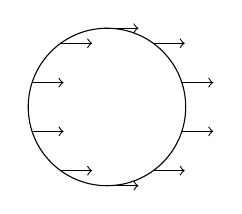
\begin{tikzpicture}
\draw (0,0) circle (1cm);
\foreach \rot in {36,72,...,360}{
\draw[->] ({sin(\rot)},{cos(\rot)}) -- +(.4,0);}
\end{tikzpicture}

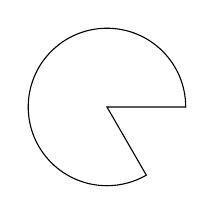
\begin{tikzpicture}
\draw (0,0) -- (1,0) arc (0:300:1cm) -- cycle;
\end{tikzpicture}

If the connection is metric compatible, the \ueig{metric is parallel transported}. This means parallel transport preserves properties like norm, orthogonality etc.

\subsection{Geodesics}
Two way of seeing it:
\begin{enumerate}
\item Parallel transports it's own tangent vector
\item Shortest distance between two points.
\end{enumerate}

\subsubsection{As a curve that parallel transports it's tangent vector}
Setting directional covariant derivative of $\od{x^\mu}{\lambda}$ to zero gives
\[ \frac{D}{d\lambda}\od{x^\mu}{\lambda} = \boxed{ \od[2]{x^\mu}{\lambda} + \Gamma^\mu_{\rho\sigma}\od{x^\rho}{\lambda}\od{x^\sigma}{\lambda} = 0 } \]
This is the \textbf{geodesic equation}. In flat space using Cartesian coordinates, this reduces to the equation of straight lines.

Actually this procedure constrains the parametrisation of the curve. In general a curve may be thought of as a geodesic if it parallel transports the \emph{unit} tangent vector. The in formula above the norm of the tangent vector was also forced to be constant. This constrains the parametrisation to be an \udef{affine parameter}, which is a parameter of the form
\[ \lambda = a\tau + b \]
with $\tau$ the arc length (i.e. proper time) and $a$ and $b$ constants.

Now say $\alpha$ is an arbitrary parametrisation and $v(\alpha) = \left|\od{x^\mu}{\alpha}\right|$ the norm of the tangent vector $\od{x^\mu}{\alpha}$. The unit tangent vector is then $v^{-1}\od{x^\mu}{\alpha}$. Requiring that this be parallel transported gives
\begin{align}
\frac{D}{d\alpha}\left(v^{-1}\od{x^\mu}{\alpha}\right) &= \od{x^\rho}{\alpha}\nabla_\rho\left[v^{-1}\od{x^\mu}{\alpha}\right] \\
&= \od{x^\rho}{\alpha} \left[\partial_\rho \left(v^{-1}\od{x^\mu}{\alpha}\right) + \Gamma^\mu_{\rho\sigma}v^{-1}\od{x^\sigma}{\alpha}\right] \\
&= \od{x^\rho}{\alpha} \left[\od{x^\mu}{\alpha}\partial_\rho v^{-1} + v^{-1}\partial_\rho \od{x^\mu}{\alpha} + \Gamma^\mu_{\rho\sigma}v^{-1}\od{x^\sigma}{\alpha}\right] = 0.
\end{align}
Multiplying both sides by $v$ gives
\[ 0 = \od{x^\mu}{\alpha}v\od{x^\rho}{\alpha}\partial_\rho v^{-1} + \od[2]{x^\mu}{\alpha} + \Gamma^\mu_{\rho\sigma}\od{x^\rho}{\alpha}\od{x^\sigma}{\alpha} \]
which is the geodesic equation derived above plus an extra term of the form $f(\alpha)\od{x^\mu}{\alpha}$, with
\begin{align}
f(\alpha) &= v \od{v^{-1}}{\alpha} \\
&= -v^{-1}\od{v}{\alpha} \\
&= - \left(\od[2]{\tau}{\alpha}\right)\left(\od{\tau}{\alpha}\right)^{-1}
\end{align}
using $v = \od{\tau}{\alpha}$, because the proper time is the arc length (TODO rephrase?). The factor $f(\alpha)$ is obviously zero for affine parameters.

For timelike paths we can write the geodesic equation in terms of the four-velocity $u^\mu = \od{x^\mu}{\tau}$:
\[ u^\lambda\nabla_\lambda u^\mu = 0 \]

For massive particles the four-momentum $p^\mu$ is $mu^\mu$, making this equivalent to
\[ p^\lambda\nabla_\lambda p^\mu = 0 \]

\subsubsection{As the shortest distance between two points}
\paragraph{For timelike paths.} Consider the proper time functional for a timelike path parametrised by $\lambda$:
\[ \tau_{AB} = \int \left(-g_{\mu\nu} \od{x^\mu}{\lambda}\od{x^\nu}{\lambda}\right)^{1/2} \diff{\lambda} \]
We want to find the stationary paths, with $\delta \tau = 0$. Computing the variation and setting $f = g_{\mu\nu} \od{x^\mu}{\lambda}\od{x^\nu}{\lambda}$ gives
\begin{align}
\delta \tau &= \int \delta\sqrt{-f}\diff{\lambda} \\
&= -\int \frac{1}{2}(-f)^{-1/2}\delta f \diff{\lambda}.
\end{align}

Now we can reparametrise the path, taking the proper time as the new parameter. This means the tangent vector is the four-velocity $u^\mu$, which fixes $f$
\[ f = g_{\mu\nu} \od{x^\mu}{\tau}\od{x^\nu}{\tau} = g_{\mu\nu}u^\mu u^\nu = -1, \]
so
\[ \delta \tau = - \frac{1}{2}\int\delta f \diff{\tau} \]

This means stationary paths of the proper time functional are also stationary paths of the simpler integral
\[ I = \frac{1}{2}\int f \diff{\tau} = \frac{1}{2}\int g_{\mu\nu} \od{x^\mu}{\tau}\od{x^\nu}{\tau} \]
and vice versa.

We can explicitly vary this integral with (TODO why)
\[ \begin{cases}
x^\mu \to x^\mu _ \delta x^\mu \\
g_{\mu\nu} \to g_{\mu\nu} + (\partial_\sigma g_{\mu\nu})\delta x^\sigma.
\end{cases} \]
Plugging this into the expression for $I$ and keeping only terms that are first order in $\delta x^\mu$, we get
\[ \delta I = \frac{1}{2}\int \left[\partial_\sigma g_{\mu\nu}\od{x^\mu}{\tau}\od{x^\nu}{\tau}\delta x^\sigma + g_{\mu\nu}\od{(\delta x^\mu)}{\tau}\od{x^\nu}{\tau} +g_{\mu\nu}\od{x^\mu}{\tau}\od{(\delta x^\nu)}{\tau}\right]\diff{\tau} \]
The last two terms can be integrated by parts; for example,
\begin{align}
\int \left[ g_{\mu\nu}\od{x^\mu}{\tau}\od{(\delta x^\nu)}{\tau} \right]\diff{\tau} &= \left. g_{\mu\nu}\od{x^\mu}{\tau}\delta x^\nu \right|_\text{at boundary} - \int \od{}{\tau}\left(g_{\mu\nu}\od{x^\mu}{\tau}\right)\delta x^\nu \diff{\tau} \\
&= - \int \left[g_{\mu\nu} \od[2]{x^\mu}{\tau} + \od{g_{\mu\nu}}{\tau}\od{x^\mu}{\tau}\right]\delta x^\nu \diff{\tau} \\
&= - \int \left[g_{\mu\nu} \od[2]{x^\mu}{\tau} + \partial_\sigma g_{\mu\nu}\od{x^\sigma}{\tau}\od{x^\mu}{\tau}\right]\delta x^\nu \diff{\tau}
\end{align}
where we have used that $\delta x^\nu$ vanishes at the boundary.

The total variation is then
\[ \delta I = - \int \left[g_{\mu\sigma}\od[2]{x^\mu}{\tau} + \frac{1}{2}\left(\partial_\mu g_{\nu\sigma} + \partial_\nu g_{\sigma\mu} - \partial_\sigma g_{\mu\nu}\right)\od{x^\mu}{\tau}\od{x^\nu}{\tau}\right]\delta x^\sigma \diff{\tau}. \]
Since we are searching for stationary points, we want $\delta I$ to vanish for any variation $\delta x^\sigma$. This implies that the expression inside the square brackets must vanish. Multiplying it with the inverse metric $g^{\rho\sigma}$ yields
\[ \od[2]{x^\rho}{\tau} + \frac{1}{2}g^{\rho\sigma}\left(\partial_\mu g_{\nu\sigma} + \partial_\nu g_{\sigma\mu} - \partial_\sigma g_{\mu\nu}\right)\od{x^\mu}{\tau}\od{x^\nu}{\tau} = 0 \]
Which is exactly the geodesic equation with the Christoffel symbols as the connection.

This procedure provides a convenient way to calculate the Christoffel symbols for a given metric: by explicitly varying the integral $I$ with the metric of interest plugged in.

\paragraph{Null geodesics.} The geodesic formula was found using a very specific parametrisation, which is not a problem because all regular curves can be arc parametrised. Unfortunately we also restricted ourselves to timelike paths, because for null paths $\tau = 0$.

Now the geodesic equation derived above is still perfectly valid, even if $\tau$ can no longer be considered a valid parameter. An affine parameter is now any parameter such that the geodesic equation is satisfied, but now there is no special one. They are all related by the fact that if $\lambda$ is an affine parameter, any parameter of the form $a\lambda + b$ is as well. 

It is often convenient to normalise the affine parameter $\lambda$ along a null geodesic such that
\[ p^\mu = \od{x^\mu}{\lambda} \]

\paragraph{Timelike geodesics are maxima.} Locally that is. We can see that this is true because any timelike path can be arbitrarily well approximated by a null curve.

\subsubsection{Exponential map}
TODO

Geodesically incomplete

Riemann normal coordinates

\subsection{Riemann curvature tensor}
We now want an object that embodies our idea of curvature. Seeing as we are going to define a new object to fit out intuition, we need to flesh it out a bit first. We begin by naming some properties of flat spacetime:
\begin{itemize}
\item Parallel transport around a closed loop leaves vectors unchanged;
\item Covariant derivatives of tensors commute;
\item Initially parallel geodesics remain parallel.
\end{itemize}
TODO motivation.
\udef{Riemann tensor $\tensor{\mathcal{R}}{^\rho_{\sigma\mu\nu}}$} is a $(1,3)$-tensor. It is antisymmetric in the last two indices.

\begin{align}
[\nabla_\mu,\nabla_\nu]V^\rho &= \nabla_\mu\nabla_\nu V^\rho - \nabla_\nu\nabla_\mu V^\rho \\
&= \left(\partial_\mu(\nabla_\nu V^\rho) - \Gamma^\lambda_{\mu\nu}\nabla_\lambda V^\rho + \Gamma^\rho_{\mu\sigma}\nabla_\nu V^\rho \right) - \left(\partial_\nu(\nabla_\mu V^\rho) - \Gamma^\lambda_{\nu\mu}\nabla_\lambda V^\rho + \Gamma^\rho_{\nu\sigma}\nabla_\mu V^\rho \right) \\
&= 2\left(\partial_{[\mu}(\nabla_{\nu]} V^\rho) - \Gamma^\lambda_{[\mu\nu]}\nabla_\lambda V^\rho + \Gamma^\rho_{[\mu|\sigma|}\nabla_{\nu]} V^\rho \right) \\
&= 2\left(\partial_{[\mu}\partial_{\nu]} V^\rho + \partial_{[\mu}(\Gamma^\rho_{\nu]\sigma} V^\sigma) - \Gamma^\lambda_{[\mu\nu]}\nabla_\lambda V^\rho + \Gamma^\rho_{[\mu|\sigma|}\partial_{\nu]} V^\sigma + \Gamma^\rho_{[\mu|\sigma|}\Gamma^\rho_{\nu]\sigma} V^\sigma \right) \\
&= \cancel{[\partial_{\mu}, \partial_{\nu}] V^\rho} + 2\left(\partial_{[\mu}(\Gamma^\rho_{\nu]\sigma} V^\sigma) - \Gamma^\lambda_{[\mu\nu]}\nabla_\lambda V^\rho + \Gamma^\rho_{[\mu|\sigma|}\partial_{\nu]} V^\sigma + \Gamma^\rho_{[\mu|\sigma|}\Gamma^\rho_{\nu]\sigma} V^\sigma \right) \\
&= 2\left(\partial_{[\mu}(\Gamma^\rho_{\nu]\sigma}) V^\sigma + \cancel{\partial_{[\mu}( V^\sigma)\Gamma^\rho_{\nu]\sigma}} - \Gamma^\lambda_{[\mu\nu]}\nabla_\lambda V^\rho + \cancel{\Gamma^\rho_{[\mu|\sigma|}\partial_{\nu]} V^\sigma} + \Gamma^\rho_{[\mu|\sigma|}\Gamma^\rho_{\nu]\sigma} V^\sigma \right) \\
&= 2\left(\partial_{[\mu}\Gamma^\rho_{\nu]\sigma} + \Gamma^\rho_{[\mu|\sigma|}\Gamma^\rho_{\nu]\sigma} \right) V^\sigma - 2\Gamma^\lambda_{[\mu\nu]}\nabla_\lambda V^\rho \\
&= \left(\partial_{\mu}\Gamma^\rho_{\nu\sigma} - \partial_{\nu}\Gamma^\rho_{\mu\sigma} + \Gamma^\rho_{\mu\sigma}\Gamma^\rho_{\nu\sigma} - \Gamma^\rho_{\nu\sigma}\Gamma^\rho_{\mu\sigma} \right) V^\sigma - \tensor{T}{^\lambda_{\mu\nu}}\nabla_\lambda V^\rho \\
&\equiv \tensor{\mathcal{R}}{^\rho_{\mu\nu\sigma}}V^\sigma - \tensor{T}{^\lambda_{\mu\nu}}\nabla_\lambda V^\rho
\end{align}

Where $[\;,\;]$ is the antisymmetrisation, $[\mu|\sigma|\nu]$ means that only $\mu$ and $\nu$ are antisymmetrised and $T$ is the torsion tensor. So the Riemann tensor is identified as
\[ \boxed{\tensor{\mathcal{R}}{^\rho_{\mu\nu\sigma}} \equiv \partial_{\mu}\Gamma^\rho_{\nu\sigma} - \partial_{\nu}\Gamma^\rho_{\mu\sigma} + \Gamma^\rho_{\mu\sigma}\Gamma^\rho_{\nu\sigma} - \Gamma^\rho_{\nu\sigma}\Gamma^\rho_{\mu\sigma}} \]

\subsubsection{Properties of the curvature tensor}
To investigate the properties of the Riemann tensor, the upper index is lowered
\[ \mathcal{R}_{\rho\sigma\mu\nu} = g_{\rho\lambda}\tensor{\mathcal{R}}{^\lambda_{\sigma\mu\nu}} \]
and an explicit expression is obtained in locally inertial coordinates. In locally inertial coordinates the metric and its first derivatives vanish, so the Christoffel symbols do as well, but not their derivatives.
\begin{align}
\mathcal{R}_{\hat{\rho}\hat{\sigma}\hat{\mu}\hat{\nu}} &= g_{\hat{\rho}\hat{\lambda}} \left(\partial_{\hat{\mu}}\Gamma^{\hat{\lambda}}_{\hat{\nu}\hat{\sigma}} - \partial_{\hat{\nu}}\Gamma^{\hat{\lambda}}_{\hat{\mu}\hat{\sigma}}\right) \\
&= \frac{1}{2}g_{\hat{\rho}\hat{\lambda}}g^{\hat{\lambda}\hat{\tau}}\left[\left(\partial_{\hat{\mu}}\partial_{\hat{\nu}}g_{\hat{\sigma}\hat{\tau}} + \partial_{\hat{\mu}}\partial_{\hat{\sigma}}g_{\hat{\tau}\hat{\nu}} - \partial_{\hat{\mu}}\partial_{\hat{\tau}}g_{\hat{\nu}\hat{\sigma}}\right) - \left(\partial_{\hat{\nu}}\partial_{\hat{\mu}}g_{\hat{\sigma}\hat{\tau}} + \partial_{\hat{\nu}}\partial_{\hat{\sigma}}g_{\hat{\tau}\hat{\mu}} - \partial_{\hat{\nu}}\partial_{\hat{\tau}}g_{\hat{\mu}\hat{\sigma}}\right)\right] \\
&= \frac{1}{2}\left[\partial_{\hat{\mu}}\partial_{\hat{\sigma}}g_{\hat{\rho}\hat{\nu}} - \partial_{\hat{\mu}}\partial_{\hat{\rho}}g_{\hat{\nu}\hat{\sigma}} - \partial_{\hat{\nu}}\partial_{\hat{\sigma}}g_{\hat{\rho}\hat{\mu}} + \partial_{\hat{\nu}}\partial_{\hat{\rho}}g_{\hat{\mu}\hat{\sigma}}\right]
\end{align}
This derivation was done in a special coordinate system, but all tensorial equations that follow from it must be true in any coordinate system. A few such equations are now listed:
\begin{enumerate}
\item The Riemann tensor is antisymmetric in its first two indices.
\[ \boxed{ \mathcal{R}_{\rho\sigma\mu\nu} = - \mathcal{R}_{\sigma\rho\mu\nu} } \]
\item The Riemann tensor is antisymmetric in its last two indices.
\[ \boxed{ \mathcal{R}_{\rho\sigma\mu\nu} = - \mathcal{R}_{\rho\sigma\nu\mu} } \]
\item The Riemann tensor is invariant under exchange of the first and last pair of indices.
\[ \boxed{ \mathcal{R}_{\rho\sigma\mu\nu} = \mathcal{R}_{\mu\nu\rho\sigma} } \]
\item Thus sum of cyclic permutations of the last three indices vanishes.
\[ \mathcal{R}_{\rho\sigma\mu\nu} + \mathcal{R}_{\rho\mu\nu\sigma} + \mathcal{R}_{\rho\nu\sigma\mu} = 0 \]
This is equivalent to the vanishing of the antisymmetric part of the last three indices.
\[ \boxed{  \mathcal{R}_{\rho[\sigma\mu\nu]} = 0 } \]
\end{enumerate}
\paragraph{Number of parameters.} TODO
\paragraph{Bianchi identity.} TODO
\[ \nabla_{[\lambda}\mathcal{R}_{\rho\sigma]\mu\nu} = 0 \]

\subsubsection{Derived quantities}
Tricks for decomposition: taking contractions and taking (anti)symmetric parts.

\paragraph{Ricci tensor.} This \udef{Ricci tensor} is defined as
\[ \mathcal{R}_{\mu\nu} \equiv \tensor{\mathcal{R}}{^\lambda_{\mu\lambda\nu}}. \]
The Ricci tensor associated with the Christoffel connection is automatically symmetric:
\begin{align}
\mathcal{R}_{\mu\nu} &= g^{\rho\lambda}\mathcal{R}_{\rho\mu\lambda\nu} = g^{\rho\lambda}\mathcal{R}_{\lambda\nu\rho\mu} = \tensor{\mathcal{R}}{^\rho_{\nu\rho\mu}} \\
&= \mathcal{R}_{\nu\mu}
\end{align}
The trace of the Ricci tensor is called the \udef{Ricci scalar} (or curvature scalar):
\[ R \equiv \tensor{\mathcal{R}}{^\mu_\mu} = g^{\mu\nu}\mathcal{R}_{\mu\nu} \]

Now a useful form of the Bianchi identity can be obtained by multiplying it by $3g^{\nu\sigma}g^{\mu\lambda}$:
\begin{align}
0 &= 3g^{\nu\sigma}g^{\mu\lambda}\nabla_{[\lambda}\mathcal{R}_{\rho\sigma]\mu\nu} \\
&= \frac{3g^{\nu\sigma}g^{\mu\lambda}}{6!}\left[\left(\nabla_{\lambda}\mathcal{R}_{\rho\sigma\mu\nu} + \nabla_{\rho}\mathcal{R}_{\sigma\lambda\mu\nu} + \nabla_{\sigma}\mathcal{R}_{\lambda\rho\mu\nu}\right) - \left(\nabla_{\lambda}\mathcal{R}_{\sigma\rho\mu\nu} + \nabla_{\rho}\mathcal{R}_{\lambda\sigma\mu\nu} + \nabla_{\sigma}\mathcal{R}_{\rho\lambda\mu\nu}\right)\right] \\
&= g^{\nu\sigma}g^{\mu\lambda}\left[\nabla_{\lambda}\mathcal{R}_{\rho\sigma\mu\nu} + \nabla_{\rho}\mathcal{R}_{\sigma\lambda\mu\nu} + \nabla_{\sigma}\mathcal{R}_{\lambda\rho\mu\nu}\right] \\
&= \nabla^\mu\mathcal{R}_{\rho\mu} - \nabla_\rho R + \nabla^\nu\mathcal{R}_{\rho\nu}
\end{align}
or
\[ \boxed{\nabla^\mu\mathcal{R}_{\rho\mu} = \frac{1}{2}\nabla_\rho R.} \]


\paragraph{Weyl tensor.} TODO Why. In $n$ dimensions the \udef{Weyl tensor} is given by
\[ C_{\rho\sigma\mu\nu} \equiv \mathcal{R}_{\rho\sigma\mu\nu} - \frac{2}{n-2}\left(g{\rho[\mu}\mathcal{R}_{\nu]\sigma} - g{\sigma[\mu}\mathcal{R}_{\nu]\rho}\right) + \frac{2}{(n-1)(n-2)}g{\rho[\mu}\mathcal{R}_{\nu]\sigma} \]
TODO properties.

\paragraph{Einstein tensor.} The \udef{Einstein tensor} is defined as
\[ G_{\mu\nu} \equiv \mathcal{R}_{\mu\nu} - \frac{1}{2}Rg_{\mu\nu}. \]
Now the Bianchi identity reduces to
\[ \boxed{\nabla^{\mu}G_{\mu\nu} = 0} \]


\section{Isometries}
\subsection{About isometries}
TODO post geometry.
\[ g'_{\mu\nu}(y) = g_{\mu\nu}(y) \]

Symmetries of arbitrary tensor fields.
\subsection{Lie derivatives}
In general $g_{\mu\nu}(x_p)$ is different from $g_{\mu\nu}(x_q)$. Are there directions we can move in on the manifold so that the metric (or any other function on the manifold) doesn't change.
So we want
\[ g_{\mu\nu}(\tilde{x}) = \pd{x^\rho}{\tilde{x}{^\mu}}\pd{x^\sigma}{\tilde{x}{^\nu}}g_{\rho\sigma}(x) \]
to equal the original metric.

We consider an infinitessimal transformation:
\[ \tilde{x}^\mu = x^\mu+\epsilon V^\mu \]
\[ \delta y^\mu = \pd{y^\mu}{x^\nu}\delta x^\nu \]

\subsubsection{Lie derivative on a scalar}
We are comparing
\[  \begin{cases}
\phi(\tilde{x}) = \phi(x + \epsilon V) = \phi(x) + \epsilon V^\mu\partial_\mu \phi(x) + \mathcal{O}(\epsilon^2) \\
\tilde{\phi}(\tilde{x}) = \phi(x)
\end{cases}\]

\begin{align}
L_V\phi &\equiv \lim_{\epsilon\to 0}\frac{\phi(\tilde{x}) - \tilde{\phi}(\tilde{x})}{\epsilon} \\
&= \lim_{\epsilon\to 0}\frac{\phi(x+\epsilon V^\mu)-\phi(x)}{\epsilon} \\
&= \lim_{\epsilon\to 0}\frac{\cancel{\phi(x)}+\epsilon V^\mu\partial_\mu\phi(x)+\mathcal{O}(\epsilon^2)-\cancel{\phi(x)}}{\epsilon} \\
&= V^\mu\partial_\mu\phi(x)
\end{align}

Ordinary directional derivative.

In general:
\[ L_V: (p,q) \text{forms} \to (p,q) \text{forms} \]

\subsubsection{Lie derivative of a vector field}
Again we define
\[ L_VW^\mu \equiv \lim_{\epsilon\to 0}\frac{W^\mu(\tilde{x}) - \tilde{W^\mu}(\tilde{x})}{\epsilon} \]
Again we are comparing two quantities
\begin{align}
W(\tilde{x}) &= W(x + \epsilon V) = W(x) + \epsilon V^\mu\partial_\mu W(x) + \mathcal{O}(\epsilon^2) \\
\tilde{W}(\tilde{x}) &= \pd{\tilde{x}^\mu}{x^\nu}W^\nu (x) \\
&= \pd{(x^\mu+\epsilon V^\mu)}{x^\nu}W^\nu (x) \\
&= \left(\delta^\mu_\nu+\epsilon \pd{V^\mu}{x^\nu}\right)W^\nu (x) \\
&= W^\mu (x)+\epsilon W^\nu (x)\partial_\nu V^\mu
\end{align}

Putting everything together, we get
\[ L_V W^\mu = V^\nu\partial_\nu W^\mu - W^\nu \partial_\nu V^\mu \]

Normal derivative not covariant, but here same as covariant derivative (extra bits cancel).

Not defined with respect to any particular metric.

Some properties:
\begin{itemize}
\item Partial derivatives can be replaced by covariant ones.
\item The Lie derivative is antisymmetric in $V$ and $W$ and defines a commutator
\[ [V,W]^\mu \equiv L_VW^\mu = - L_WV^\mu \]
This satisfies the Jacobi identity 
\[ [V,[W,X]]^\mu + [X,[V,W]]^\mu + [W,[X,V]]^\mu \]
and thus is a Lie bracket.  The Jacobi identity is equivalent to
\[ L_V[W,X]^\mu = [L_VW,X]^\mu + [W,L_VX]^\mu \]
\end{itemize}


\subsubsection{Lie derivative of other tensor fields}
The definitions above are readily generalised
\[ \tilde{x}^\mu(x) = x^\mu +\epsilon V^\mu(x) \]
\[ L_VT = \lim_{\epsilon\to 0} \frac{T(\tilde{x})-\tilde{T}(\tilde{x})}{\epsilon} \]
where we need
\[ \pd{\tilde{x}^\mu}{x^\rho} = \delta^\mu_\rho + \epsilon \partial_\rho V^\mu + \mathcal{O}(\epsilon^2) \qquad \text{and}\qquad \pd{x^\mu}{\tilde{x}{^\rho}} = \delta^\mu_\rho - \epsilon \partial_\rho V^\mu + \mathcal{O}(\epsilon^2) \]

Again partial derivatives can be replaced by covariant derivatives. We illustrate with a $(0,2)$-tensor $T_{\mu\nu}$.
\[ \begin{cases}
T_{\mu\nu}(\tilde{x}) = T_{\mu\nu}(x) + \epsilon V^\rho\partial_\rho T_{\mu\nu}+ \mathcal{O}(\epsilon^2) \\
\tilde{T}_{\mu\nu}(\tilde{x}) = \pd{x^\mu}{\tilde{x}{^\mu}}\pd{x^\nu}{\tilde{x}{^\nu}}T_{\mu\nu} = T_{\mu\nu} - \epsilon\partial_\mu V^\rho T_{\rho\nu}(x) - \epsilon\partial_\nu V^\sigma T_{\mu\sigma} + \mathcal{O}(\epsilon^2)
\end{cases} \]
Filling this in gives
\begin{align}
L_V T_{\mu\nu} &= \lim_{\epsilon\to 0} \frac{T_{\mu\nu}(\tilde{x})-\tilde{T}_{\mu\nu}(\tilde{x})}{\epsilon} \\
&= \lim_{\epsilon\to 0} \frac{\cancel{T_{\mu\nu}(x)}+\epsilon V^\rho\partial_\rho T_{\mu\nu}+ \mathcal{O}(\epsilon^2)-\cancel{T_{\mu\nu}}+\epsilon T_{\rho\nu} \partial_\mu V^\rho +\epsilon T_{\mu\sigma} \partial_\nu V^\sigma + \mathcal{O}(\epsilon^2)}{\epsilon} \\
&= V^\rho\partial_\rho T_{\mu\nu} + T_{\rho\nu} \partial_\mu V^\rho + T_{\mu\rho} \partial_\nu V^\rho \\
&= V^\rho \left(\nabla_\rho T + \Gamma^\lambda_{\rho \mu}T_{\lambda \nu} + \Gamma^\lambda_{\rho \nu}T_{\mu \lambda} \right) + T_{\rho\nu} \left(\nabla_\mu V^\rho - \Gamma^\rho_{\mu\lambda}V^\lambda\right) + T_{\mu\rho} \left(\nabla_\nu V^\rho - \Gamma^\rho_{\nu\lambda}V^\lambda\right) \\
&= V^\rho\nabla_\rho T + T_{\rho\nu}\nabla_\mu V^\rho + T_{\mu\rho}\nabla_\nu V^\rho + \left(\Gamma^\lambda_{\rho \mu}V^\rho T_{\lambda \nu} - \Gamma^\rho_{\mu\lambda}V^\lambda T_{\rho\nu}\right) + \left(\Gamma^\lambda_{\rho \nu}V^\rho T_{\mu \lambda} - \Gamma^\rho_{\nu\lambda}V^\lambda T_{\mu\rho}\right) \\
&= V^\rho\nabla_\rho T + T_{\rho\nu}\nabla_\mu V^\rho + T_{\mu\rho}\nabla_\nu V^\rho
\end{align}

Isometries from an algebra
\[ \left[L_V,L_W\right] = L_{[V,W]} \]
Enough to verify scalars and vectors.

\subsubsection{Lie derivative of tensor densities}
TODO

\subsection{Killing vectors}
The Lie derivative of the metric tensor. This is $(0,2)$-tensor, so the formula is the one given above.
Due to metric compatibility, the first term is zero
\begin{align}
L_V g_{\mu\nu} &= V^\rho\nabla_\rho g_{\mu\nu} + g_{\lambda\nu}\nabla_\mu V^\lambda + g_{\mu\lambda}\nabla_\nu V^\lambda \\
&= g_{\lambda\nu}\nabla_\mu V^\lambda + g_{\mu\lambda}\nabla_\nu V^\lambda \\
&= \nabla_\mu V_\nu + \nabla_\nu V_\nu \\
\end{align}

An infinitesimal coordinate transformation is a symmetry of the metric if $L_V g_{\mu\nu} = 0$, which is equivalent to requiring $V$ to satisfy the equations
\[ \nabla_\mu V_\nu + \nabla_\nu V_\nu = 0 = \nabla_{(\mu} V_{\nu)}. \]
Such vectors are called \udef{Killing vectors}. These equations are equivalent to
\[ \nabla_\mu V_\nu = \nabla_{[\mu}V_{\nu]} \]


Properties:
\begin{enumerate}
\item Killing vectors form a Lie algebra. If $V$ and $W$ are Killing vectors, i.e. $L_Vg_{\mu\nu} = L_Wg_{\mu\nu} = 0$, then $[V,W]$ is a Killing vector because
\[ L_{[V,W]}g_{\mu\nu} = L_VL_Wg_{\mu\nu} - L_WL_V g_{\mu\nu} = 0  \]
\item If all the components of the metric are independent of a particular coordinate, say $y$
\[ \partial_y g_{\mu\nu} \qquad \forall \mu,\nu \]
Then $V=\partial_y$ is a Killing vector. A coordinate system in which a Killing vector is a partial derivative is said to be \textit{adapted} to the Killing vector (or isometry) in question. TODO derive Killing equations from this.
\item Two Killing vectors commute if and only if there is a coordinate system that is adapted to both of them.
\end{enumerate}

You can use the equations in 2 ways:
\begin{itemize}
\item Impose symmetries on the metric.
\item Find the Killing vectors for a given metric, which gives the symmetries
\end{itemize}

\begin{example}
Algebra of Killing vectors in Minkowski and two-sphere.
\end{example}

\subsection{Conserved quantities}
\subsubsection{Conserved charges along geodesics}
Let $K^\mu$ be a Killing vector field and $x^\mu(\tau)$ a geodesic with four-velocity $x^\mu$. Then the quantity
\[ Q_K = K_\mu u^\mu \]
is constant along the geodesic. Indeed,
\begin{align}
\od{}{\tau}Q_K = \od{K_\mu u^\mu}{\tau} &= u^\mu \od{K_\mu}{\tau} + K_\mu \od{}{\tau}u^\mu \\
&= u^\mu u^\nu \nabla_\nu K_\mu + 0\\
&= \frac{1}{2}\left(\nabla_\nu K_\mu + \nabla_\mu K_\nu\right)u^\mu u^\nu = 0
\end{align}
where the last equality is due to the Killing equations.

\subsubsection{Conserved currents from the energy-momentum tensor}
Let $K^\mu$ be a Killing vector field and $T^{\mu\nu}$ the covariantly conserved symmetric energy-momentum tensor ($\nabla_\mu T^{\mu\nu} = 0$). Then the current
\[ J_K^\mu = T^{\mu\nu}K_\nu \]
is covariantly conserved. Indeed,
\begin{align}
\nabla_\mu J^\mu_K &= (\nabla_\mu T^{\mu\nu})K_\nu + T^{\mu\nu} \nabla_\mu K_\nu \\
&= 0 + \frac{1}{2}T^{\mu\nu}\left(\nabla_\mu K_\nu + \nabla_\nu K_\mu\right) = 0
\end{align}

\subsubsection{Komar currents}
The Einstein tensor is symmetric and conserved (from the Bianchi identity), so we have the conserved current
\[ J^\mu_1 = \tensor{G}{^\mu_\nu}K^\nu =  \]

\subsection{Killing tensors}

\subsubsection{Killing(-Stäckel) tensors}
A \udef{Killing tensor $K_{\beta_1\ldots\beta_n}$} is a totally symmetric tensor satisfying
\[ \nabla_{(\alpha}K_{\beta_1\ldots\beta_n)} = 0. \]

The charge
\[ Q_K = K_{\beta_1\ldots\beta_n}u^{\beta_1}\ldots u^{\beta_n} \]
is constant along the geodesic.

\subsubsection{Killing-Yano tensors}
A \udef{Killing-Yano tensor $Y_{\beta_1\ldots\beta_n}$} is a totally anti-symmetric tensor satisfying
\[ \nabla_{(\alpha} Y_{\beta_1)\ldots\beta_n} = 0 \qquad \text{or, equivalenty} \qquad \nabla_\alpha Y_{\beta_1\ldots\beta_n} = \nabla_{[\alpha}Y_{\beta_1\ldots\beta_n]} \]

The tensorial charges
\[ Z_{\beta_1\ldots\beta_{n-1}} = u^\beta Y_{\beta\beta_1\ldots\beta_{n-1}} \]
are conserved along geodesics.


\subsubsection{Symmetries and conserved charges (Komar integrals)}
\subsubsection{Conservation laws}
Conservation laws
\begin{itemize}
\item for geodesics
\item for spacetime
\end{itemize}

\[ Q = V^\mu \od{x^\nu}{\tau}g_{\mu\nu} \]
$\od{}{\tau}Q$ if $V$ is Killing and $\dot{x}^\mu$ is a geodesic.
\begin{align}
\od{}{\tau}Q = \od{}{\tau}\left(V_\mu\dot{x}^\mu\right) &= \left(\frac{DV_\mu}{D\tau}\right)\dot{x}^\mu + V_\mu \frac{D\dot{x}^\mu}{\tau} \\
&= \underbrace{\dot{x}^\rho D_\rho V_\mu \dot{x}^\mu}_{=0 \text{because Killing}} + \underbrace{V_\mu \frac{D\dot{x}^\mu}{D\tau}}_{=0 \text{geodesic}}
\end{align}

\subsection{Maximally symmetric spaces}
In D=4, maximally 10 symmetries. Minkowski maximally symmetric, but not uniquely so.
(Depends on number of killing vectors (which also form an algebra and can commute or not))

\[ K^\mu(x) \text{Killing} \quad \Leftrightarrow \quad D_{[\mu}K_{\nu]} = 0 \]
\[ K_\mu(x) = K_\mu(x^*) + \partial_\nu K_\mu(x^*)(x^\nu-x^{\nu*}) + \frac{1}{2}\partial_\rho\partial_\nu K_\mu(x^*)(x^\nu-x^{\nu *}(x^\rho - x^{\rho*}) + \ldots \]

\[ D_\mu K_\nu = \partial_\mu K_\nu - \Gamma^\rho_{\mu\nu}K_\rho \]
\[ \partial_\nu K_\mu(x^*) = D_\nu K_\mu(x^*) + \Gamma_{\nu\mu}^{\;\;\rho}K_\rho(x^*) \]
With
\[ D_\nu K_\mu(x^*) = \underbrace{\cancel{D_{(\nu}K_{\mu)}}}_{0 \text{because Killing}} + D_{[\nu}K_{\mu]}(x^*) \]
So
\[ \frac{D(D-1)}{2} \qquad \text{for} D=4 \quad \Rightarrow \quad 6 \text{coeff.} \]

Maximally symmetric:
\begin{itemize}
\item Minkowski: 4 translations, 6 Lorentz ($\Lambda = 0$)
\[ [P_\mu, P_\nu] = 0, \qquad [M_{\mu\nu}, P_\rho] = 2 \eta_{\rho[\mu}P_{\nu]}, \qquad [M_{\mu\nu}, M^{\rho\sigma}] = 4 \delta_{[\mu}^{\;\;[\rho}M_{\nu]}^{\;\;\sigma]} \]
\[M^{\mu\nu} = x^\mu\partial^\nu - x^\nu\partial^\mu \qquad G=\R^4 \rtimes \SO(1,3)\]
\item de Sitter $G = \SO(1,4)$ ($\Lambda>0$)
\item Anti-de Sitter $G=\SO(2,3)$
\end{itemize}
On a side note
\[ dS_4 \equiv \frac{\SO(1,4)}{\SO(1,3)} \qquad AdS_4 \equiv \frac{\SO(2,3)}{\SO(1,3)} \]
Confer:
\[ S^p = \frac{\SO(p+1)}{\SO(p)} \]

riemann normal coordinates + freely falling frames

\section{Conformal transformations}
\subsection{Conformal Killing vectors}
\[ L_C g_{\mu\nu} = \nabla_\mu C_\nu + \nabla_\nu C_\mu = 2\omega(x)g_{\mu\nu} \]

A Killing vector for a metric is at least a conformal Killing vector for any conformally rescaled metric.

\subsubsection{Conserved charges along null geodesics}
\[ Q_C = C_\mu u^\mu \]
\subsubsection{Conserved currents from the energy-momentum tensor}
energy-momentum tensor is traceless
\[ J_C^\mu = T^{\mu\nu}C_\nu \]

\subsection{Conformal Killing(-Yano) tensors}


\chapter{Lie groups and algebras}

\section{Lie Group}
A Lie group is a topological group that is also a differential manifold. This means we can apply differentials, which is of course very important. So important in fact that Sophus Lie called Lie groups infinitesimal groups when he first introduced them. Not only that, but it means we can consider tangent spaces, which will also be important later. TODO better justification

Bearing in mind the link between the topology and group properties explored in the section on topological groups, we quite naturally arrive at the following definition:
\begin{definition}
A \udef{Lie group} is a smooth manifold $G$ which is also a group and such that both the group product $G\times G \to G$ and the inverse map $G \to G$ are smooth.
\end{definition}

There is a particular type of Lie group that will be of particular importance to us, namely the matrix Lie group. In fact we will almost exclusively consider matrix Lie groups.

\subsection{Matrix Lie group}
For matrix groups there is a simpler condition to see whether it is a Lie group or not:
\begin{eigenschap}
All \ueig{closed subgroups} of $\GL(n, \C)$ are matrix Lie groups.
\end{eigenschap}
The condition that it be closed means that for every sequence in the Lie group the limit needs to be in the Lie group as well, if there is one. (Or you can say every Cauchy sequence in the Lie group has to have a limit in the Lie group). This is a technicality and is satisfied for most of the interesting subgroups of $\GL(n, \C)$. 

We have already seen that all subgroups of $\GL(n, \C)$ are topological groups. To prove the assertion then we must only verify that it is a smooth manifold. Because $\C^{n\times n}$ is a manifold and a matrix Lie group is a subset of $\C^{n\times n}$, the matrix Lie group inherits Hausdorffness and second-countability from $\C^{n\times n}$. To show it is smooth and locally homeomorphic to $\R^{m}$ in every point, we will explicitly construct such homeomorphisms using the matrix exponential.

\subsubsection{Exponential maps}
The homeomorphisms will be constructed based on the exponential map.
\[ \exp: \GL(n,\C) \to \GL(n,\C): X \mapsto e^X \]
This map is not a bijection, however if we restrict it to a neighbourhood of $\mathbb{0}$, it is locally a bijection. In fact it maps that neighbourhood to a neighbourhood of $\mathbb{1}$. More formally
\begin{eigenschap}
There exists a neighbourhood $U$ of $\mathbb{0}$ and a neighbourhood $V$ of $\mathbb{1}$ such that the exponential mapping takes $U$ homeomorphically onto $V$.
\end{eigenschap}
This result should not be surprising. For $X$ close to $\mathbb{0}$ we have the approximation $e^{X} \approx \mathbb{1} + X + \mathcal{O}(X^2)$. So for matrices in a small neighbourhood $U$ around $\mathbb{0}$ the exponential mapping can be seen as approximately linear, which is injective. In order to get surjectivity, we restrict the codomain of the mapping to the image of $U$ under the exponential mapping. This is a neighbourhood of $\mathbb{1}$ because $e^0 = \mathbb{1}$. 

We have obtained a bijection and because the matrix exponential is continuous, this restriction of it is also continuous. We would now like to show that the map maps open sets in our matrix Lie group, which we shall now call $G$, to open sets of $\R^{m}$. Unfortunately it doesn't. There is no reason why $\mathbb{0}$ or any matrices in $U$ should be elements of $G$. (Remember that the relevant group operation for matrix groups is the matrix multiplication, for which the neutral element is $\mathbb{1}$; the matrix $\mathbb{0}$ is of no particular importance in this context.) Being a group, the matrix Lie group must contain $\mathbb{1}$; being a topological group, it must contain a neighbourhood of $\mathbb{1}$; being a subspace of $\GL(n,\C)$ endowed with the subspace topology, the intersection of $V$ with that neighbourhood is an open set in $G$ which we will call $V'$.

So if we invert the restricted matrix exponential, we get a homeomorphism from \undline{one} neighbourhood of $G$ to $\GL(n,\C)$, which can then be composed with a homeomorphism to $\R^m$.

\begin{definition}
The inverse map $\exp^{-1}: V' \to U$ is called the \udef{logarithm}.
\end{definition}

From this we can construct a homeomorphism from a neighbourhood of any element $A$ of $G$. By multiplying each element of $V'$ with $A$ we get a neighbourhood $V_A$ of $A$. We define the following homeomorphism on $V_A$: multiply by $A^{-1}$ (this is bijective due to associativity of the group operation and continuous due to the definition of topological groups) and then send through the inverted, restricted matrix exponential. This composition of homeomorphisms is a homeomorphism. So for each element $A \in G$ we can find a neighbourhood $V_A$ that is homeomorphic to $\R^m$ thanks to this homeomorphism.

\begin{example}
TODO Finite Lie group
\end{example}


\subsubsection{Lie algebra of a matrix Lie group}
TODO: justification

\begin{definition}
Let $G$ be a matrix Lie group. The \udef{Lie algebra} of $G$, denoted $\mathfrak{g}$, is the set of all matrices $X_t$ such that $e^{itX_t}$ is in $G$ for all \undline{\textbf{real}} numbers $t$. We call the matrices $X_t$ \udef{generators} of the group.
\end{definition}

\begin{note}
Now here we have a complication. There are actually two conventions. The definition above is the convention most often used in physics. In the mathematics literature the Lie algebra in usually defined using $e^{tX_t}$, not $e^{itX_t}$. The physics convention gives rise to Hermitian generators in the algebras of $\U(n)$ and $\SU(n)$. This is useful because we are often interested in turning them into quantum operators, which correspond to observables only if they are Hermitian. The downside of this convention however is that it makes our life much more difficult in other places, and it even means that some definitions don't make any sense. In what follows we will generally be using the physics convention. We will however make use of the mathematics convention when the need arises. Also if there are interesting differences in the mathematics definition, we will mention those as well.
\end{note}

To try to grasp why the definition given above is useful, we introduce the notion of parametrization of group elements.
\subsubsection{Parametrization of group elements.}
When first introducing the matrix groups, we pointed out how the elements could be written in function of real parameters. We now make this notion more concrete and begin by defining a one-parameter subgroup.
\begin{definition}
A function $A : \R \to \GL(n, \C)$ is called a \udef{one-parameter subgroup} of $\GL(n, \C)$ if
\begin{enumerate}
\item $A$ is continuous,
\item $A(0) = \mathbb{1}_n$,
\item $A(t+s) = A(t)A(s)$ for all $t,s \in \R$.
\end{enumerate}
\end{definition}
If $A$ is a one-parameter subgroup of $\GL(n,\C)$, then it has the following property:
\begin{eigenschap}
There exists a unique $n\times n$ complex matrix $X$ such that
\[ A(t) = e^{tX} \]
\end{eigenschap}

So $X_t$ is in $\mathfrak{g}$ if and only if the one-parameter subgroup generated by $X_t$ lies in G. Conversely for any one-parameter subgroup that is a subgroup of G, there exists a generator and that generator is by definition part of the algebra.

Before continuing we shall consider some examples of algebras of matrix Lie groups. In general we shall call the algebra of a Lie group the lowercase version of the name of the Lie group. E.g., the Lie algebra of $\GL(n, \C)$ is $\glAlg(n,\C)$.

\begin{example}
\begin{enumerate}
\item If $X$ is any $n\times n$ complex matrix, then $e^{itX}$ is invertible. Thus the Lie algebra, $\glAlg(n,\C)$, of the invertible matrices, $\GL(n,\C)$, is the space of all complex $n\times n$ matrices.
\item If we use the mathematical convention, then the Lie algebra of $\GL(n,\R)$ is the space of all real $n\times n$ matrices, denoted $\glAlg(n,\R)$. To prove this we first remark that is $X$ is any real $n\times n$ matrix, then $e^{tX}$ will be invertible and real. Conversely, if $e^{tX}$ is real for all real $t$, then $X=\left.\od{}{t}e^{tX}\right|_{t=0}$ will also be real. Obviously in the physics convention the above no longer holds true.

\item The Lie algebra $\slAlg(n,\C)$ of $\SL(n,\C)$ is the space of all complex $n \times n$ matrices with zero trace. To prove this we use that
\[ \det(e^X) = e^{\Tr(X)}. \]
If $\Tr(X) = 0$, then $\det(e^{itX}) = 1$ for all real numbers $t$. On the other hand, if $X$ is any $n\times n$ matrix such that $\det(e^{itX}) =1$ for all $t$, then $e^{it\Tr(X)} = 1$ for all $t$. This means that $it\Tr(X)$ is an integer multiple of $2\pi i$ for all $t$, which is only possible if $\Tr(X) = 0$.

\item Lie algebra of $\U(N)$. If $X$ is to be a generator in our algebra, we need $e^{itX}$ to be unitary. So
\[ \left(e^{itX}\right)^\dagger = \left(e^{itX}\right)^{-1} = e^{-itX}. \]
We also have that
\[ \left(e^{itX}\right)^\dagger = e^{-itX^\dagger}. \]
Which gives us
\[ e^{-itX} = e^{-itX^\dagger}. \]
Differentiating at $t=0$ we see that the generators have to be Hermitian ($X = X^\dagger$).

We can also prove this by writing out the definition of the matrix exponential. 
\[ U(N) \ni U = e^{it_iX_i} \]
\begin{align}
\mathbb{1} = U^\dagger U &= (\mathbb{1}-it_i X_i^\dagger + \ldots )(\mathbb{1}+it_i X_i + \ldots) \\
&= \mathbb{1} + it_i(X_i^\dagger - X_i) + \ldots = \mathbb{1}
\end{align}
So we require the generators to be Hermitian matrices ($X_i^\dagger = X_i$). We have $N^2$ independent $X_i$ that are Hermitian. 
\[ \uAlg(N) = \{ H \in \GL(N,\C), H^\dagger = H \} \]
In the mathematics convention this condition becomes that the generators have to be skew-Hermitian, i.e. $X_i^\dagger = -X_i$.

\item Lie algebra of $\SU(N)$. Combining the arguments for the algebras of the unitary and special linear group, we see that the generators must be unitary and of trace zero. In other words the algebra is given by
\[ \suAlg(N) = \{ H\in\uAlg(N), \Tr[H] = 0 \} \]
and has dimension $N^2-1$.

For $N=2$ we have:
\[ \begin{cases}
\suAlg(2) = \{\sigma_1, \sigma_2, \sigma_3\} \\
\uAlg(2) = \{\sigma_1, \sigma_2, \sigma_3, \mathbb{1}\}
\end{cases} \]
Where
\[ \sigma_1 = \begin{pmatrix}
0 & 1 \\ 1 & 0
\end{pmatrix}, \qquad \sigma_2 = \begin{pmatrix}
0 & -i \\ i & 0
\end{pmatrix}, \qquad \sigma_3 = \begin{pmatrix}
1 & 0 \\ 0 & -1
\end{pmatrix}\]

\item Lie algebra of $\Ogroup(N)$. As explained above, if we want the algebra to be real, we need to make use of the mathematical convention. So $O=e^{t_iX_i}$.
\begin{align}
\mathbb{1} = O^\intercal O = e^{t_iX_i^\intercal}e^{t_iX_i} &= (\mathbb{1}+t_i X_i^\intercal + \ldots )(\mathbb{1}+t_i X_i + \ldots) \\
&= \mathbb{1} + t_i(X^\intercal_i + X_i) + \ldots
\end{align}
So we require the generators to be antisymmetric matrices ($X_i^\intercal = -X_i$).
\[ \oAlg(N) = \{ X \in \GL(N,\R), X^\intercal = -X \} = \soAlg(N) \]
The dimension of $\oAlg(N)$ is $\frac{N(N-1)}{2}$.
\end{enumerate}
\end{example}

The Lie algebra as defined above is in some way prototypical. I.e. when we make this notion more abstract, we want the abstract notion to behave in a similar fashion and have many of the same properties. Of course to do that we first need an idea of what properties these Lie algebras actually have. This is what we will be exploring next.

\begin{eigenschap}
If $G$ is a \textit{connected} matrix Lie group, then every $A \in G$ can be written in the form
\[ A = e^{X_1}e^{X_2}\ldots e^{X_m} \]
for some $X_1, X_2, \ldots, X_m$ in $\mathfrak{g}$
\end{eigenschap}

\begin{eigenschap}
Every continuous homomorphism between two matrix Lie groups is smooth.
\end{eigenschap}

\begin{eigenschap}
A matrix $X$ is in $\mathfrak{g}$ if and only if there exists a smooth curve $\gamma$ in $\C^{n\times n}$ such that
\begin{enumerate}
\item $\gamma(t)$ lies in $G$ for all $t$;
\item $\gamma(0) = \mathbb{1}$;
\item $\left.\od{\gamma}{t}\right|_{t=0} = X$
\end{enumerate}
Thus $\mathfrak{g}$ is the tangent space at the identity to $G$.
\end{eigenschap}


\begin{itemize}
\item If we assume $X \in \mathfrak{g}$, we can take $\gamma(t) = \exp(tX)$. This $\gamma(t)$ satisfies the points of the proposition above.
\item We now assume $\gamma(t)$ is a smooth curve in $G$ with $\gamma(0) = \mathbb{1}$.
\begin{align}\od{\gamma(t)}{t} &= \lim_{\delta t \to 0} \frac{\gamma(t+\delta t)-\gamma(t)}{\delta t} = \gamma(t)\left(\lim_{\delta t \to 0}\frac{\gamma(\delta t)-\gamma(0)}{\delta t}\right) \\ &= \gamma(t)\left.\od{\gamma}{t}\right|_{t=0} = \gamma(t)X \end{align}
From which we get that
\[ \gamma(t) = \exp{tX} \]
\end{itemize}

Now this is interesting, so interesting in fact that we use this last proposition to construct a general definition of a Lie algebra associated to a Lie group.

We can now also reintroduce the physics convention. We just divide all elements of any algebra by the imaginary unit $i$. The elements of this algebra may not be closed under the bracket operation, but that does not matter as we have a different definition to work from now: they are elements of the tangent space at identity to $G$, rescaled with a fractor $-i$.

We have already seen that in the mathematics convention the commutator belongs to the algebra (remembering to sum according to Einstein notation):
\[ [X_i, X_j] = f_{ij}^k X_k \]
Where we call $f_{ij}^k$ a \udef{structure constant} (with respect to the chosen basis of course). In the physics convention, we obviously need to deal with the factor $i$:
\[ [X_i, X_j] = if_{ij}^k X_k \]
\begin{eigenschap}
From the antisymmetry of the bracket we get:
\[ f^k_{ij} + f^k_{ji} = 0 \]
From the Jacobi identity we get:
\[ f^m_{ie}f^e_{jk} + f^m_{je}f^e_{ki} + f^m_{ke}f^e_{ij} = 0 \]
\end{eigenschap}

And lastly a final property of Lie algebras of matrix Lie groups follows straight from the \ueig{Baker-Campbell-Hausdorff formula}: 
\[ e^{A}e^{B} = e^C \qquad \text{with} \qquad C=A+B+\frac{1}{2}[A,B] + \frac{1}{12}([A,[A,B]]+[B,[B,A]]) + \ldots  \]
\begin{eigenschap}
To know the (local) structure of a Lie group close to the identity one \ueig{only} needs to know the commutator of the generators $[X_i,X_j]$
\end{eigenschap}

\section{Lie Algebra}
Again we will start by restricting our attention to Lie algebra's of matrix Lie groups. That way we can give some examples that will (hopefully) aid in the understanding of the general case.


\subsection{Definition}

\begin{eigenschap}
Let $G$ be a matrix Lie group, with Lie algebra $\mathfrak(g)$. Let $X$ and $Y$ be elements of $\mathfrak{g}$. Then
\begin{enumerate}
\item $sX \in \mathfrak{g}$, for all \undline{real} numbers $s$,
\item $X+Y \in \mathfrak{g}$,
\item $-i(XY - YX)\in \mathfrak{g}$.
\end{enumerate}
\end{eigenschap}
The first two points mean that the Lie algebra is actually a vector space over the \undline{real} numbers. This is important and serves as the crux of our first generalisation of Lie algebras, so we will have a quick look at the proofs of the statements above. 

\begin{enumerate}
\item This first point is fairly straightforward, since $e^{t(sX)} = e^{(ts)X}$, which must be in $G$ if $X$ is in $\mathfrak{g}$.
\item If $X$ and $Y$ commute, this is again immediate. If they don't however we need to do a little more work. We start from the Lie product formula:
\[ e^{t(X+Y)} = \lim_{m\to\infty} \left(e^{\frac{tX}{m}}e^{\frac{tY}{m}}\right)^m \]
Clearly if $X, Y \in \mathfrak{g}$,  for every $m$, $e^{\frac{tX}{m}}$ and $e^{\frac{tY}{m}}$ are elements of $G$. Since $G$ is a group, $\left(e^{\frac{tX}{m}}e^{\frac{tY}{m}}\right)^m$ is in $G$. Now because $G$ is a matrix Lie group, and thus \textit{closed} in $\GL(n, \C)$, the limit must also be in $G$. (If that is the limit is in $\GL(n, \C)$, which it is because $e^{t(X+Y)}$ is invertible). This shows that $X+Y$ is in $\mathfrak{g}$.
\item The third point follows from the product rule of the differential operator. Alternatively we can use the Baker-Campbell-Hausdorff formula:
\[e^{tX}e^{sY} = e^{tX+sY+ \frac{ts}{2}[X,Y] + \ldots}\]
This together with the first two points shows the third point.
\end{enumerate}

We have shown that the Lie algebra is a vector space over the real numbers, but crucially a Lie algebra is in general not a vector space over complex numbers, even if it consists of matrices with complex entries. For an example we consider the algebra $\suAlg(n)$, which consists of Hermitian matrices with zero trace. Assume $X$ is such a matrix. Now because $(iX)^\dagger = -iX^\dagger = -iX$, $iX$ is not Hermitian. As a consequence it cannot be an element of $\suAlg(n)$ and thus $\suAlg(n)$ is not a complex vector space.

If we follow the mathematical definition, the third point becomes $XY - YX \in \mathfrak{g}$. This will be important later. In fact it's so important we will give it name.
\begin{definition}
Given two $n \times n$ matrices $A$ and $B$, the \udef{bracket} (or \udef{commutator}) of $A$ and $B$, denoted $[A,B]$ is defined to be
\[ [A,B] = AB - BA \]
\end{definition}

Using the mathematical convention, the Lie algebra of any matrix Lie group is closed under brackets. This is in general not the case using the physics convention. Take for example the algebra $\suAlg(2)$, generated by $\{\sigma_1, \sigma_2, \sigma_3\}$. Then
\[ [\sigma_1,\sigma_2] = \begin{pmatrix}
2i & 0 \\ 0 & -2i
\end{pmatrix} \]
which is not Hermitian and thus not an element of $\suAlg(2)$! This also means that $\suAlg(n)$ (with $n>1$) is not an algebra in according to the definition we are about to give.

Despite the problems with the conventions, these properties seem nice. We would like to study things that exhibit these properties in general. So based on this we define a Lie algebra in general in the following way.

\begin{definition}
A (finite-dimensional) real or complex \udef{Lie algebra $\mathfrak{g}$} is an $n$-dim (real or complex) vector space with the following map:
\[[\cdot,\cdot]: \mathfrak{g}\times\mathfrak{g} \to \mathfrak{g}: (X,Y) \mapsto [X,Y]\]
that has the following properties
\begin{enumerate}
\item Bilinear: $\forall X,Y,Z \in \mathfrak{g}, \qquad a,b \in \R \quad (\text{or} \C)$:
\[ [aX + bY, Z] = a[X,Z] + b[Y,Z] \]
\item Antisymmetric: $\forall X,Y \in \mathfrak{g}$
\[ [X,Y] = -[Y,X] \]
\item Satisfies the \udef{Jacobi identity}: $\forall X,Y,Z \in \mathfrak{g}$
\[ [X,[Y,Z]] + [Y,[Z,X]] + [Z,[X,Y]] = 0 \]
\end{enumerate}
\end{definition}
The only surprising thing in this definition is the appearance of the Jacobi identity. It can be thought of as a condition that takes the place of associativity, but is weaker. In fact every Lie algebra can be embedded in into some associative algebra so that the bracket corresponds to the operation $XY - YX$. 

If we follow the mathematical convention, the Lie algebra of a matrix Lie group is a real Lie algebra in the sense of the above definition. Unfortunately this is not true for the physics convention.

As noted above, this notably means $\suAlg(n)$ (with $n>1$) is not an algebra in according this definition. There are several ways to solve this problem. The obvious one would be to redefine the bracket operator when using the physics convention (i.e. say that $[A,B] = -i \left(AB - BA\right)$). This is usually not done. We could also extend $\suAlg(n)$ to include $iX$ for every $X \in \suAlg(n)$ (this is called the \udef{complexification} of $\suAlg(n)$), which would mean that $\suAlg(n)$ is actually $\slAlg(n)$ (i.e. we drop the condition that the elements of $\suAlg(n)$ have to be Hermitian). This is apparently actually done sometimes in the physics literature. Or finally we can do what we will do in these notes, namely forget about this definition, use the definition we will motivate in the next section and write the extra $i$ whenever it pops up.

Furthermore for every finite-dimensional real or complex vector space $V$, let $\glAlg(V)$ denote the space of linear maps of $V$ into itself. Then $\glAlg(V)$ is a real or complex Lie algebra with the bracket operation $[A,B] = AB - BA$.

\subsection{Lie algebra of a Lie group}

We finally define the Lie algebra:
\begin{definition}
The \udef{Lie algebra} of a Lie group $G$ is the tangent space at the identity with the bracket operation defined by
\[ [v,w] = [X^v, X^w]_e. \]
\end{definition}



\section{Representations of Lie algebras}
TODO: representations of Lie groups: Representation vs linear group action. Continuous groups must be represented on the physical Hilbert space by unitary operators $U(T(\theta))$.


We start with some definitions.

\begin{definition}
A \udef{homomorphism} between two algebras $\mathfrak{g}_1, \mathfrak{g}_2$ is a map that preserves $[,]$:
\[ \phi: \mathfrak{g}_1 \to \mathfrak{g}_2: [X_1,X_2] \mapsto \phi([X_1,X_2]) = [\phi(X_1), \phi(X_2)] \]
If the map is invertible, it is called an \udef{isomorphism}.
\end{definition}

Every Lie group homomorphism gives rise to a Lie algebra homomorphism.
\begin{eigenschap}
Let $G$ and $H$ be matrix Lie groups, with Lie algebras $\mathfrak{g}$ and $\mathfrak{h}$ respectively. Suppose that $\Phi: G \to H$ is a Lie group homomorphism. Then there exists a unique real linear \ueig{homomorphism} $\phi: \mathfrak{g} \to \mathfrak{h}$ such that
\[\Phi\left(e^{X}\right) = e^{\phi(X)}\]
for all $X \in \mathfrak{g}$. The map $\phi$ has the following additional properties:
\begin{enumerate}
\item $\phi\left(AXA^{-1}\right) = \Phi(A)\phi(X)\Phi(A)^{-1}$, for all $X\in\mathfrak{g}, A \in G$
\item $\phi(X) = \left.\od{}{t}\Phi \left(e^{tX}\right)\right|_{t=0}$, for all $X \in \mathfrak{g}$
\end{enumerate}
\end{eigenschap}

\begin{definition}
An \udef{algebra representations} is a homomorphism between an abstract algebra and the space of linear operators.
\[ D: \mathfrak{g} \to \GL(n,\R) \; \text{or} \; \GL(n,\C): X \mapsto D(X) \]
A representation is said to be faithful if it is injective.
\end{definition}

\begin{eigenschap}
\ueig{Ado's theorem}:
Any finite dimensional Lie algebra admits a faithful matrix representation.
\end{eigenschap}
This nontrivial theorem means that every Lie algebra can be viewed as a subalgebra of $\glAlg(n,\C)$, and thus as an algebra of a matrix Lie group.

\subsection{Adjoint representation}

\begin{eigenschap}
Let $G$ be a matrix Lie group, with Lie algebra $\mathfrak(g)$. Let $X$ be an element of $\mathfrak{g}$ and $A$ an element of $G$.
\[ AXA^{-1} \in \mathfrak{g} \]
\end{eigenschap}
This means that the following definition makes sense:
\begin{definition}
Let $G$ be a matrix Lie group with algebra $\mathfrak{g}$. Then for each $A \in G$ we define the linear map $\Ad_A: \mathfrak{g} \to \mathfrak{g}$ by the formula
\[ \Ad_A(X) = AXA^{-1} \]
\end{definition}
\begin{eigenschap}
\begin{itemize}
\item $\Ad_A^{-1} = \Ad_{A^{-1}}$.
\item The map $A \to \Ad_A$ is a group homomorphism of $G$ into $\GL(\mathfrak{g})$.
\item $\Ad_A([X,Y]) = [\Ad_A(X),\Ad_A(Y)] \qquad \forall A\in G, X,Y \in \mathfrak{g}$.
\end{itemize}
\end{eigenschap}
Because $A \to \Ad_A$ is a group homomorphism, we have an associated algebra homomorphism, $X \mapsto \ad_X$.
\begin{eigenschap}
The associated Lie algebra map $\ad: \mathfrak{g} \to \glAlg(\mathfrak{g})$ is given by
\[ \ad_X(Y) = [X,Y] \]
\end{eigenschap}
This last property generalises well and we can use it to define the adjunct map for a Lie algebra in general.

The maps $\Ad$ and $\ad$ give the \udef{adjoint representations} of $G$ and $\mathfrak{g}$.

The adjoint representation $\ad_{X_i}$ is linear, and thus can be represented as a matrix. So for every $X_i$ in the basis, we have a $T_i$ that maps the coordinates of a $Y \in \mathfrak{g}$ to $[X_i, Y]$. If we write $Y = c_1X_1 + c_2X_2 + c_3X_3 + \ldots$, then
\[ T_i \begin{pmatrix}
c_1 \\ c_2 \\ \vdots
\end{pmatrix} = \begin{pmatrix}
if^1_{11}c_1 + if^1_{12}c_2 + \hdots \\
if^2_{11}c_1 + if^2_{12}c_2 + \hdots \\
\vdots
\end{pmatrix} \]
So
\[ T_i = \begin{pmatrix}
if^1_{11} & if^1_{12} & \ldots \\
if^2_{11} & if^2_{12} & \ldots \\
\vdots
\end{pmatrix} \qquad \text{or} \qquad \left(T_i\right)^k_j = if^k_{ij}\]
These matrices have the following property (derived from the Jacobi identity):
\begin{eigenschap}
\[ [T_i,T_j] = -if_{ij}^k T_k \]
\end{eigenschap}
 

\begin{definition}
The \udef{Cartan-Killing form} 
\begin{align}
g_{ij} &\equiv \Tr[T_i\cdot T_j] \\
&=-f_{ik}^ef_{je}^k
\end{align}
\end{definition}

\begin{definition}
The \udef{quadratic Casimir} in a given representation of an algebra is given by
\[ C_2 = g^{ij}X_iX_j \]
This is an \ueig{invariant} for a specific representation.
\end{definition}

\begin{eigenschap}
The quadratic Casimir \ueig{commutes} with any element $X$ of the algebra:
\[ [C_2,X] = 0 \]
In general $C_2 \notin \mathfrak{g}$
\end{eigenschap}
A \udef{Casimir} is an operator that commutes with all generators. 
\begin{example}
The angular momentum operators have to structure of $\suAlg(2)$
\begin{align}
[L_i,L_j] &= i\epsilon_{ijk}L_k \qquad (L_i \; \text{generators}) \\
[L^2, L_i] &= 0
\end{align}
\end{example}

\begin{example}
Find the Casimir operator of the fundamental representation of $\suAlg(2)$.

We call $\tau_i = \frac{\sigma_i}{2}$, so that
\[ [\tau_i, \tau_j] = i\epsilon_{ijk}\tau_k \]
We then compute
\begin{align}
C_2 &= \sum_{i,j}g^{ij}\tau_i\tau_j = \frac{1}{2}\sum_{i,j}\delta_{ij}\tau_i\tau_j = \frac{3}{8}\mathbb{1} \\
&= \frac{1}{2}s(s+1) \mathbb{1} \qquad \Rightarrow \qquad s= \tfrac{1}{2}
\end{align}
Where we used that $g^{ij} = (g_{ij})^{-1}$ and $g_{ij} = \epsilon_{ike}\epsilon_{jke} = 2\delta_{ij}$
\end{example}

\subsection{Representations of $\suAlg(2)$}
\subsubsection{The algebras $\suAlg(2)$ and $\soAlg(3)$} are isomorphic
\[ \soAlg(3) = \{ X\in \GL(3,\R), X^\intercal = -X \} \]
\[ X_1 = \begin{pmatrix}
0 & 0 & 0 \\ 0 & 0 & 1 \\ 0 & -1 & 0
\end{pmatrix}, \qquad X_2 = \begin{pmatrix}
0 & 0 & -1 \\ 0&0&0 \\ 1&0&0
\end{pmatrix}, \qquad X_3 = \begin{pmatrix}
0&1&0 \\ -1&0&0 \\ 0&0&0
\end{pmatrix} \]

\begin{example}
Show that $[X_i,X_j] = -\epsilon_{ijk}X_k$
\end{example}

Let $J_i$ be
\[ J_i = -iX_i \]
so that $[J_i,J_j] = i\epsilon_{ijk}J_k$. Then $J_i$ are generators of $\suAlg(2)$.
\remark{The groups have the same algebra, which means they are the same around identity}
\subsubsection{Building the $\suAlg(2)$ representation} we run into the problem that the $J_i$ cannot be diagonalised simultaneously, i.e. they don't commute.
So we choose a basis in which $J_3$ is diagonal, then we define
\[ J_\pm \equiv J_1 \pm iJ_2 \]
With the following properties:
\[ \begin{cases}
[J_3,J_\pm] = [J_3,J_1]\pm i[J_3,J_2] = iJ_2 \pm J_1 = \pm J_\pm \\
[J_+, J_-] = i[J_2,J_1] - i[J_1,J_2] = 2J_3
\end{cases} \]
We now notate a basis of states $V$ with $\ket{j,m}$
\[ J_3\ket{j,m} = m\ket{j,m} \]
where $m$ is an eigenvalue of $J_3$ and $j$ is the biggest eigenvalue ($m\leq j$). We can find enough eigenvectors to make the basis because $J_3$ is diagonal.

From the relation 
\begin{align}
J_3 \left(J_\pm\ket{j,m}\right) &= \left(J_\pm J_3 + [J_3,J_\pm]\right)\ket{j,m} \\
&= J_\pm m \ket{j,m} \pm J_\pm \ket{j,m} \\
&= (m\pm 1)\left(J_\pm\ket{j,m}\right)
\end{align}
we get the following
\[ \begin{cases}
J_+\ket{j,j} = 0 \qquad (j>0) \\
J_-\ket{j,j_-} = 0 \qquad (j_- \;\text{smallest eigenvalue of}\; J_3)
\end{cases} \]

We also see that the eigenvalues are spaced an integer apart, from $j_-$ to $j$.


Because the trace of a commutator is zero (as the trace is cyclic), we also have that 
\[ \Tr[J_3] = \frac{1}{2}\Tr([J_+,J_-]) = 0 = \sum_{j_-}^j m \]
which means that
\[ 0 = j + (j-1) + \ldots + (j_-+1) +j_- \quad \Rightarrow \quad j+j_- = 0 \quad \Rightarrow \quad j_- = -j \]

So the dimension of $V$ is $2j+1$, which must be an integer, meaning that $j$ must be half-integer.

We also impose the following normalisation:
\[ \braket{j,m} = 1 \qquad \braket{j,j} = 1\]

For a generic state $\ket{j,m}$ we get the following:
\begin{align}
J_3\ket{j,m} &= m\ket{j,m} \\
J_+\ket{j,m} &= [(j+1+m)(j+m)]^{1/2} \ket{j,m+1} \\
J_-\ket{j,m} &= [(j+1-m)(j+m)]^{1/2} \ket{j,m-1}
\end{align}

\begin{example}
Fundamental representation of $\suAlg(2)$ (i.e. of dimension $2$).

\[ j=1/2 \qquad \begin{cases}
\ket{1/2,+1/2} = \begin{pmatrix} 1 \\ 0 \end{pmatrix} \\
\ket{1/2,-1/2} = \begin{pmatrix} 0 \\ 1 \end{pmatrix}
\end{cases} \]
\[ J_3 = - \frac{1}{2} \begin{pmatrix}
-1 & 0 \\ 0 & 1
\end{pmatrix} = \frac{\sigma_3}{2} \]
\[ \begin{cases}
J_+\ket{1/2, 1/2} = 0 \\ J_+\ket{1/2, -1/2} = \ket{1/2,1/2}
\end{cases} \qquad \begin{cases}
J_-\ket{1/2, 1/2} = \ket{1/2,-1/2} \\ J_-\ket{1/2, -1/2} = 0
\end{cases} \]
\[J_+ = \begin{pmatrix}
0&1\\0&0
\end{pmatrix} \qquad J_- = \begin{pmatrix}
0&0\\1&0
\end{pmatrix}\]
\[ J_1 = \frac{1}{2}\begin{pmatrix}
0&1\\1&0
\end{pmatrix} = \frac{\sigma_2}{2} \qquad J_2 = \frac{1}{2} \begin{pmatrix}
0&-i\\i&0
\end{pmatrix} = \frac{\sigma_2}{2}\]
\end{example}

\begin{example}
The $j=1$ representation of $\suAlg(2)$
\[\ket{1,1} = \begin{pmatrix} 1\\0\\0 \end{pmatrix}, \quad \ket{1,0} = \begin{pmatrix} 0\\1\\0 \end{pmatrix}, \quad \ket{1,-1} = \begin{pmatrix} 0\\0\\1 \end{pmatrix} \quad J_3 = \begin{pmatrix}
1&0&0\\0&0&0\\0&0&-1
\end{pmatrix}\]
\[ \begin{cases}
J_+\ket{1,1} = 0 \\
J_+\ket{1,0} = \sqrt{2}\ket{1,1} \\
J_+\ket{1,-1} = \sqrt{2}\ket{1,0}
\end{cases} \qquad \begin{cases}
J_-\ket{1,1} = \sqrt{2}\ket{1,0} \\
J_-\ket{1,0} = \sqrt{2}\ket{1,-1} \\
J_-\ket{1,-1} = 0
\end{cases} \]
\[J_+ = \sqrt{2}\begin{pmatrix}
0&1&0\\0&0&1\\0&0&0
\end{pmatrix} \qquad J_- = \sqrt{2}\begin{pmatrix}
0&0&0\\1&0&0\\0&1&0
\end{pmatrix}\]
\[ J_1 = \frac{1}{\sqrt{2}}\begin{pmatrix}
0&1&0\\1&0&1\\0&1&0
\end{pmatrix} \qquad J_2 = \frac{1}{\sqrt{2}} \begin{pmatrix}
0&-i&0\\i&0&-i\\0&i&0
\end{pmatrix}\]
\end{example}

\begin{example}
Exercise: calculate $C_2$
\[ C_2 = \frac{1}{2}l(l+1) \qquad (l=1) \]
\end{example}

\chapter{Riemannian manifolds}
\section{Riemannian metrics}
\begin{definition}
Let $M$ be a smooth manifold. A \udef{Riemannian metric} on $M$ is a smooth covariant $2$-tensor field $g\in T^*M\otimes T^*M$ whose value $g_p$ at each point $p\in M$ is an inner product on $T_pM$. We often use the notation
\[ \inner{v,w}_g \defeq g_p(v,w) \]
where $p\in M$ and $v,w\in T_pM$. Similarly we write $\norm{v}_g \defeq \sqrt{\inner{v,v}_g}$.

A \udef{Riemannian manifold} is a pair $(M,g)$ where $M$ is a smooth manifold and $g$ is a Riemannian metric on $M$.
\end{definition}

Most things work with boundary as well.

\begin{lemma}
Every smooth manifold admits a Riemannian metric.
\end{lemma}
\begin{proof}
TODO with partition of unity.
\end{proof}

\begin{example}
The \udef{Euclidean metric} is the Riemannian metric $g_E$ on the manifold $\R^n$ whose value at each $x\in\R^n$ is the standard inner product on $T_x\R^n$.
\end{example}

\subsection{Isometries}
\begin{definition}
Let $(M_1, g_1)$ and $(M_2, g_2)$ be Riemannian manifolds. An \udef{isometry} from $(M_1, g_1)$ to $(M_2, g_2)$ is a diffeomorphism $\varphi: M_1\to M_2$ such that $\varphi^* g_2 = g_1$.

We say $\varphi: M_1\to M_2$ is a \udef{local isometry} if for each point $p\in M_1$ their is a neighbourhood $U(p)$ such that $\varphi|_U$ is an isometry onto an open subset of $M_2$.

A Riemannian $n$-manifold is called \udef{flat} if it is locally isometric to a Euclidean space.
\end{definition}
An isometry from $(M,g)$ to itself is called an isometry of $(M,g)$. The set of isometries of $(M,g)$ is a group under composition, the \udef{isometry group} of $(M,g)$, denoted $\Iso(M,g)$.

\begin{lemma}
All Riemannian $1$-manifolds are flat.
\end{lemma}

\begin{lemma}
A mapping $\varphi:M\to M'$ between smooth manifolds is an isometry \textup{if and only if} $\varphi$ is a smooth bijection and each differential $\diff\varphi_p:T_pM\to T_{\varphi(p)}M'$ is a linear isometry.
\end{lemma}
\begin{proof}
The only part to prove is that $\varphi$ is automatically a diffeomorphism if it is a smooth bijection. This follows from the global rank theorem \ref{globalRank} because $F$ has contant rank (equal to the dimension of $M$ and $M'$).
\end{proof}

\subsection{Local representations for metrics}
Let $(x^1, \ldots, x^n)$ be smooth local coordinates on the neighbourhood $U\subseteq M$. Then $g|_U$ can be written as
\[ g|_U = g_{ij}\diff{x^i}\otimes\diff{x^j}  \]
The definition of inner product translates to the requirement that $[g(p)]_{ij}$ be a symmetric, non-singular matrix. Using symmetry we get the symmetric product
\[ g|_U = g_{ij}\diff{x^i}\diff{x^j} \]

\begin{example}
The Euclidean metric can be expressed as
\[ g_E = \sum_i\diff{x^i}\diff{x^i} = \delta_{ij}\diff{x^i}\diff{x^i} \]
so $g_{ij} = \delta_{ij}$.
\end{example}

\begin{proposition}
Given a smooth local frame for $TM$ we can construct a smooth orthonormal frame with the same span.
\end{proposition}
\begin{proof}
Gram-Schmidt.
\end{proof}

\subsection{Constructing Riemannian metrics}
\subsection{Riemannian immersions}
\begin{proposition}
Let $(M,g)$ be a Riemannian manifold, $M'$ a smooth manifold and $F:M'\to M$ a smooth map. Then $g' = F^*g$ is a Riemannian metric on $M$ \textup{if and only if} $F$ is an immersion.
\end{proposition}
\begin{proof}
The only reason $g' = F^*g$ may fail to be a metric is if it is not definite. First assume $F$ is not an immersion. Then there exist $p\in M'$ and $v,w\in T_pM'$ such that $\diff{F}_p(v) = \diff{F}_p(w)$ and $v\neq w$. Then $v-w \neq 0$, but
\[ \inner{v-w,v-w}_{g'}= \inner{\diff{F}(v-w),\diff{F}(v-w)}_{g} = \inner{0,0}_g = 0. \]
Conversely, assume $g'$ not definite. Then there exists a $v\neq 0$ such that $0 = \norm{v}_{g'}= \norm{\diff{F}(v)}_{g}$, implying $\diff{F}(v) = 0$. Thus the kernel of $\diff{F}$ is not $\{0\}$, meaning it is not injective by \ref{injectivityKernelTriviality} and thus $F$ is not an immersion by definition. 
\end{proof}
The metric $g' = F^*g$ of the proposition is called the \udef{metric induced by $F$}.

An immersion (resp. embedding) $F: (M,g)\to (M',g')$ is called an \udef{isometric immersion} (resp. \udef{isometric embedding}) if $g' = F^*g$.

\begin{lemma}
Existence of adapted orthonormal frames.
\end{lemma}

\begin{definition}
Let $(M,g)$ be a Riemannian manifold and $M'\subseteq M$ a smooth submanifold. A vector $v\in T_pM$, for some $p\in M'$, is called \udef{normal} to $M'$ if $\inner{v,w}_g = 0$ for every $w\in T_pM'$.

The space of all vectors normal to $M'$ at $p\in M'$ is called the \udef{normal space} $N_pM'$ at $p$.
\end{definition}
Clearly $N_pM' = (T_pM')^\perp$ and
\[ T_pM = T_pM' \oplus N_pM'. \]

\begin{proposition}[Normal bundle]
Let $(M,g)$ be a Riemannian $m$-manifold without boundary and $M'\subseteq M$ a an immersed $n$-submanifold. The set
\[ NM' = \bigsqcup_{p\in M'}N_pM' \]
is a smooth subbundle of $TM|_{M'}$ of rank $(m-n)$.
\end{proposition}
The vector bundle $NM'$ is called the \udef{normal bundle} of $M'$.

A section of the normal bundle $NM'$ is called a \udef{normal vector field} along $M'$.

The \udef{tangential projection} $\pi^\top: TM|_{M'}\to TM'$ and the \udef{normal projection} $\pi^\perp: TM|_{M'}\to NM'$ are the maps that for each $p\in M'$ restrict to the orthogonal projections $T_pM\to T_pM'$ and $T_pM\to N_pM'$.

\begin{lemma}
The tangential and normal projections are smooth bundle homomorphisms
\end{lemma}

\subsection{Riemannian products}
\begin{definition}
Let $(M_1,g_1)$ and $(M_2,g_2)$ be Riemannian manifolds. The product manifold $M_1\times M_2$ has a natural Riemannian metric $g=g_1\oplus g_2$ called the \udef{product metric} defined by
\[ g_{p_1,p_2}: (T_{p_1}M_1\oplus T_{p_2}M_2)^2 \to \R: (v_1+v_2, w_1+w_2) \mapsto g_1|_{p_1}(v_1,w_1) + g_2|_{p_2}(v_2,w_2) \]
where we have identified $T_{(p_1,p_2)}(M_1\times M_2)$ with $T_{p_1}M_1\oplus T_{p_2}M_2$.
\end{definition}

\subsection{Riemannian submersions}
\subsubsection{Horizontal and vertical tangent spaces}
Suppose $M,M'$ are smooth manifolds, $\pi:M\to M'$a smooth submersion and $g$ a Riemannian metric on $M$.

TODO: we can view $M$ as a fibre bundle with as fibres the properly embedded smooth manifolds $M_y = \pi^{-1}(y)$.

At each point $x\in M$ we can split $T_xM$ into two subspaces $V_x \oplus H_x$, the \udef{horizontal} and \udef{vertical tangent spaces} at $x$, defined by
\[ V_x \defeq \ker\diff{\pi}_x = T_x(M_{\pi(x)}) \qquad \text{and} \qquad H_x = (V_x)^\perp. \]
Where the equality $\ker\diff{\pi}_x = T_x(M_{\pi(x)})$ is due to (TODO tangent space to a submanifold). Notice that the definition of $V_x$ does not depend on the metric, but the definition of $H_x$ does.

A \udef{horizontal vector field} on $M$ consists of vectors in the horizontal tangent space and a \udef{vectical vector field} on $M$ consists of vectors in the vertical tangent tangent space on $M$.

A vector field $X$ on $M$ is a \udef{horizontal lift} of a vector field $X'$ on $M'$ if $X$ is horizontal and $\pi$-related to $X$, which means that
\[ \forall x\in M: \; \diff{\pi}_x(X_x) = X'_{\pi(x)} .\]

\begin{proposition}
Let $M,M'$ be smooth manifolds, $\pi:M\to M'$ a smooth submersion and $g$ a Riemannian metric on $M$.
\begin{enumerate}
\item Every smooth vector field $W$ on $M$ can uniquely be expressed as the sum of a smooth horizontal and a smooth vertical vector field:
\[ W = W^H + W^V. \]
\item Every smooth vector field on $M'$ has a unique smooth horizontal lift to $M$.
\item For every $x\in M$ and $v\in H_x$, there is a vector field $X'\in\mathfrak{X}(M')$ whose horizontal lift $X$ satisfies $X_x = v$.
\end{enumerate}
\end{proposition}
The last part of the previous proposition says that any horizontal vector can be extended to a horizontal lift on all of $M$.

Importantly, it is \emph{not true} that every horizontal vector field on $M$ is a horizontal lift.
\begin{example}
Take $\pi: \R^2\to\R: (x,y)\mapsto x$. Let $W$ be the smooth vector field $y\partial_x$ on $\R^2$. At any point $V_p= \Span\{\partial_y\}$ and $H_p= \Span\{\partial_x\}$, so $W$ is horizontal. But there is no vector field on $\R$ whose horizontal lift is $W$. Indeed $\diff{\pi}_p(W) = y\partial_x$ is not constant on $\pi^{-1}(p)$ because it depends on $y$.
\end{example}

\subsubsection{Riemannian submersions}
\begin{definition}
Let $\pi: (M,g)\to (M',g')$ be a smooth submersion between Riemannian manifolds. Then $\pi$ is a \udef{Riemannian submersion} if $\diff{\pi}_x|_{H_x}: H_x\to T_{\pi(x)}M'$ is a (bijective) linear isometry for all $x\in M$.
\end{definition}
Equivalently, the submersion $\pi$ is a Riemannian submersion if the metrics satisfy
\[ \forall x\in M:\; \forall v,w\in H_x:\; g_x(v,w) = g'_{\pi(x)}(\diff{\pi}_x(v), \diff{\pi}_x(w)). \]

\subsubsection{Riemannian coverings}

\subsection{Basic constructions derived from the metric}
\subsubsection{Raising and lowering indices}
Let $M$ be a smooth manifold. Given a Riemannian metric $g$ in $M$, we define a bundle homomorphism
\[ \hat{g}: TM \to T^*M: v\mapsto g_p(v,\cdot). \]
In other words we have $\hat{g}(v)(w) = g_p(v,w)$ for all $p\in M$ and $v,w\in T_pM$.

Musical isomorphisms

\subsubsection{Inner products of tensors}
We define $\inner{\omega, \eta}_g \defeq \inner{\omega^\sharp, \eta^\sharp}$.
Then
\[ \inner{\omega,\eta}= g_{kl}(g^{ki}\omega_i)(g^{lj}\eta_j) = \delta^i_lg^{lj}\omega_i\eta_j = g^{ij}\omega_i\eta_j. \]



\section{Connections}
\subsection{Affine connection}
\begin{definition}
Let $\pi: E\to M$ be a smooth vector bundle over a smooth manifold $M$ and let $\Gamma(E)$ denote the space of sections of $E$. A \udef{connection} in $E$ is a map
\[ \nabla: \mathfrak{X}(M)\times \Gamma(E) \to \Gamma(E): (X,Y)\mapsto \nabla_X Y \]
satisfying the following properties:
\begin{enumerate}
\item $\nabla_X Y$
\end{enumerate}
\end{definition}

\section{Geodesics}


\section{Curvature}




\chapter{Algebraic geometry}
\chapter{Geometric topology}
\section{Vector bundles}
\subsection{Definition}
\subsection{Operations on vector bundles}